%%%%%%%%%%%%%%%%%%%%%%%%%%%%%%%%%%%%%%%%%
% Masters/Doctoral Thesis 
% LaTeX Template
% Version 1.43 (17/5/14)
%
% This template has been downloaded from:
% http://www.LaTeXTemplates.com
%
% Original authors:
% Steven Gunn 
% http://users.ecs.soton.ac.uk/srg/softwaretools/document/templates/
% and••••••••
% Sunil Patel
% http://www.sunilpatel.co.uk/thesis-template/
%
% License:
% CC BY-NC-SA 3.0 (http://creativecommons.org/licenses/by-nc-sa/3.0/)
%
% Note:
% Make sure to edit document variables in the Thesis.cls file
%
%%%%%%%%%%%%%%%%%%%%%%%%%%%%%%%%%%%%%%%%% 

%----------------------------------------------------------------------------------------
%	PACKAGES AND OTHER DOCUMENT CONFIGURATIONS
%----------------------------------------------------------------------------------------

\documentclass[11pt, oneside]{Thesis} % The default font size and one-sided printing (no margin offsets)

\graphicspath{{Pictures/}} % Specifies the directory where pictures are stored

\usepackage[comma, sort&compress]{natbib} % Use the natbib reference package - read up on this to edit the reference style; if you want text (e.g. Smith et al., 2012) for the in-text references (instead of numbers), remove 'numbers' 

%\usepackage{booktabs}
%\usepackage{array}
\usepackage{amsmath,array}
\newcolumntype{L}[1]{>{\raggedright\arraybackslash}m{#1}}
%\usepackage{apacite}
\usepackage{multirow}
\usepackage{fixltx2e}
\usepackage{enumerate}
\def\SPSB#1#2{\rlap{\textsuperscript{\textcolor{red}{#1}}}\SB{#2}}
\def\SP#1{\textsuperscript{\textcolor{black}{#1}}}
\def\SB#1{\textsubscript{\textcolor{black}{#1}}}

\newcolumntype{x}[1]
            {>{\raggedright}p{#1}}
\newcommand{\tn}{\tabularnewline}

\hypersetup{urlcolor=blue, colorlinks=true} % Colors hyperlinks in blue - change to black if annoying
\title{\ttitle} % Defines the thesis title - don't touch this

\begin{document}

\frontmatter % Use roman page numbering style (i, ii, iii, iv...) for the pre-content pages

\setstretch{1.3} % Line spacing of 1.3

% Define the page headers using the FancyHdr package and set up for one-sided printing
\fancyhead{} % Clears all page headers and footers
\rhead{\thepage} % Sets the right side header to show the page number
\lhead{} % Clears the left side page header

\pagestyle{fancy} % Finally, use the "fancy" page style to implement the FancyHdr headers

\newcommand{\HRule}{\rule{\linewidth}{0.5mm}} % New command to make the lines in the title page

% PDF meta-data
\hypersetup{pdftitle={\ttitle}}
\hypersetup{pdfsubject=\subjectname}
\hypersetup{pdfauthor=\authornames}
\hypersetup{pdfkeywords=\keywordnames}

%----------------------------------------------------------------------------------------
%	TITLE PAGE
%----------------------------------------------------------------------------------------

\begin{titlepage}
\begin{center}

\textsc{\LARGE \univname}\\[1.5cm] % University name
\textsc{\Large Doctoral Thesis}\\[0.5cm] % Thesis type

\HRule \\[0.5cm] % Horizontal line
{\huge \bfseries \ttitle}\\[0.4cm] % Thesis title
\HRule \\[1.5cm] % Horizontal line

\begin{minipage}{0.4\textwidth}
\begin{flushleft} \large
\emph{Author:}\\
{\authornames} % Author name - remove the \href bracket to remove the link
\end{flushleft}
\end{minipage}
\begin{minipage}{0.4\textwidth}
\begin{flushright} \large
\emph{Supervisors:} \\
{\supname} % Supervisor name - remove the \href bracket to remove the link  
\end{flushright}
\end{minipage}\\[3cm]
 
\large \textit{A thesis submitted in fulfilment of the requirements\\ for the degree of \degreename}\\[0.3cm] % University requirement text
\textit{in the}\\[0.4cm]
\groupname\\\deptname\\[2cm] % Research group name and department name
 
{\large \today}\\[4cm] % Date
%\includegraphics{Logo} % University/department logo - uncomment to place it
 
\vfill
\end{center}

\end{titlepage}

%----------------------------------------------------------------------------------------
%	DECLARATION PAGE
%	Your institution may give you a different text to place here
%----------------------------------------------------------------------------------------

\Declaration{

\addtocontents{toc}{\vspace{1em}} % Add a gap in the Contents, for aesthetics

I, \authornames, declare that this thesis titled, '\ttitle' and the work presented in it are my own. I confirm that:

\begin{itemize} 
\item[\tiny{$\blacksquare$}] This work was done wholly or mainly while in candidature for a research degree at this University.
\item[\tiny{$\blacksquare$}] Where any part of this thesis has previously been submitted for a degree or any other qualification at this University or any other institution, this has been clearly stated.
\item[\tiny{$\blacksquare$}] Where I have consulted the published work of others, this is always clearly attributed.
\item[\tiny{$\blacksquare$}] Where I have quoted from the work of others, the source is always given. With the exception of such quotations, this thesis is entirely my own work.
\item[\tiny{$\blacksquare$}] I have acknowledged all main sources of help.
\item[\tiny{$\blacksquare$}] Where the thesis is based on work done by myself jointly with others, I have made clear exactly what was done by others and what I have contributed myself.\\
\end{itemize}
 
Signed:\\
\rule[1em]{25em}{0.5pt} % This prints a line for the signature
 
Date:\\
\rule[1em]{25em}{0.5pt} % This prints a line to write the date
}

\clearpage % Start a new page

%----------------------------------------------------------------------------------------
%	QUOTATION PAGE
%----------------------------------------------------------------------------------------

\pagestyle{empty} % No headers or footers for the following pages

\null\vfill % Add some space to move the quote down the page a bit

\textit{``Thanks to my solid academic training, today I can write hundreds of words on virtually any topic without possessing a shred of information, which is how I got a good job in journalism."}

\begin{flushright}
Dave Barry
\end{flushright}

\vfill\vfill\vfill\vfill\vfill\vfill\null % Add some space at the bottom to position the quote just right

\clearpage % Start a new page

%----------------------------------------------------------------------------------------
%	ABSTRACT PAGE
%----------------------------------------------------------------------------------------

\addtotoc{Abstract} % Add the "Abstract" page entry to the Contents

\abstract{\addtocontents{toc}{\vspace{1em}} % Add a gap in the Contents, for aesthetics

The Thesis Abstract is written here (and usually kept to just this page). The page is kept centered vertically so can expand into the blank space above the title too\ldots
}

\clearpage % Start a new page

%----------------------------------------------------------------------------------------
%	ACKNOWLEDGEMENTS
%----------------------------------------------------------------------------------------

\setstretch{1.3} % Reset the line-spacing to 1.3 for body text (if it has changed)

\acknowledgements{\addtocontents{toc}{\vspace{1em}} % Add a gap in the Contents, for aesthetics

The acknowledgements and the people to thank go here, don't forget to include your project advisor\ldots
}
\clearpage % Start a new page

%----------------------------------------------------------------------------------------
%	LIST OF CONTENTS/FIGURES/TABLES PAGES
%----------------------------------------------------------------------------------------

\pagestyle{fancy} % The page style headers have been "empty" all this time, now use the "fancy" headers as defined before to bring them back

\lhead{\emph{Contents}} % Set the left side page header to "Contents"
\tableofcontents % Write out the Table of Contents

\lhead{\emph{List of Figures}} % Set the left side page header to "List of Figures"
\listoffigures % Write out the List of Figures

\lhead{\emph{List of Tables}} % Set the left side page header to "List of Tables"
\listoftables % Write out the List of Tables

%----------------------------------------------------------------------------------------
%	ABBREVIATIONS
%----------------------------------------------------------------------------------------

\clearpage % Start a new page

\setstretch{1.5} % Set the line spacing to 1.5, this makes the following tables easier to read

\lhead{\emph{Abbreviations}} % Set the left side page header to "Abbreviations"
\listofsymbols{ll} % Include a list of Abbreviations (a table of two columns)
{
\textbf{BBM} & \textbf{B}lack \textbf{B}erry \textbf{M}essenger \\
\textbf{ICT} & \textbf{I}nformation and \textbf{C}ommunications \textbf{T}echnology \\
\textbf{MMS} & \textbf{M}ultimedia \textbf{M}essaging \textbf{S}ervice \\
\textbf{USSD} & \textbf{U}nstructured \textbf{S}upplementary \textbf{S}ervice \textbf{D}ata \\
%\textbf{Acronym} & \textbf{W}hat (it) \textbf{S}tands \textbf{F}or \\
}

%----------------------------------------------------------------------------------------
%	PHYSICAL CONSTANTS/OTHER DEFINITIONS
%----------------------------------------------------------------------------------------

\clearpage % Start a new page

\lhead{\emph{Physical Constants}} % Set the left side page header to "Physical Constants"

\listofconstants{lrcl} % Include a list of Physical Constants (a four column table)
{
Speed of Light & $c$ & $=$ & $2.997\ 924\ 58\times10^{8}\ \mbox{ms}^{-\mbox{s}}$ (exact)\\
% Constant Name & Symbol & = & Constant Value (with units) \\
}

%----------------------------------------------------------------------------------------
%	SYMBOLS
%----------------------------------------------------------------------------------------

\clearpage % Start a new page

\lhead{\emph{Symbols}} % Set the left side page header to "Symbols"

\listofnomenclature{lll} % Include a list of Symbols (a three column table)
{
$a$ & distance & m \\
$P$ & power & W (Js$^{-1}$) \\
% Symbol & Name & Unit \\

& & \\ % Gap to separate the Roman symbols from the Greek

$\omega$ & angular frequency & rads$^{-1}$ \\
% Symbol & Name & Unit \\
}

%----------------------------------------------------------------------------------------
%	DEDICATION
%----------------------------------------------------------------------------------------

\setstretch{1.3} % Return the line spacing back to 1.3

\pagestyle{empty} % Page style needs to be empty for this page

\dedicatory{For/Dedicated to/To my\ldots} % Dedication text

\addtocontents{toc}{\vspace{2em}} % Add a gap in the Contents, for aesthetics

%----------------------------------------------------------------------------------------
%	THESIS CONTENT - CHAPTERS
%----------------------------------------------------------------------------------------

\mainmatter % Begin numeric (1,2,3...) page numbering

\pagestyle{fancy} % Return the page headers back to the "fancy" style

% Include the chapters of the thesis as separate files from the Chapters folder
% Uncomment the lines as you write the chapters
% Chapter 1

\chapter{Introduction} % Main chapter title

\label{introductionchapter} % For referencing the chapter elsewhere, use \ref{Chapter1} 

\lhead{Chapter 1. \emph{Introduction}} % This is for the header on each page - perhaps a shortened title

%----------------------------------------------------------------------------------------
\section{Introduction}
 
\section{Thesis Organization}

\begin{flushright}
\end{flushright}

% Chapter 1

\chapter{Related Work} % Main chapter title

\label{relatedworkchapter} % For referencing the chapter elsewhere, use \ref{Chapter1} 

\lhead{Chapter 1. \emph{Related Work}} % This is for the header on each page - perhaps a shortened title

%----------------------------------------------------------------------------------------
\section{Persuasive Technologies}

\begin{flushright}
\end{flushright}

% Chapter 1

\chapter{Study Context} % Main chapter title

\label{contextchapter} % For referencing the chapter elsewhere, use \ref{Chapter1} 

\lhead{Chapter 1. \emph{Study Context}} % This is for the header on each page - perhaps a shortened title

%----------------------------------------------------------------------------------------
\section{Obesity in South Africa}
Most of apartheid policies towards health didn't focus towards these populations and some of the current health and economical concerns are as result of amplifications of apartheid social clusters \citep{benatar2013challenges}. 
\section{Context Description}

\begin{flushright}
\end{flushright}

% Chapter 1

\chapter{Contextual Enquiry} % Main chapter title

\label{contextualenqchapter} % For referencing the chapter elsewhere, use \ref{Chapter1} 

\lhead{Chapter 1. \emph{Contextual Enquiry}} % This is for the header on each page - perhaps a shortened title

%----------------------------------------------------------------------------------------
\section{Study Description}
The purpose of this study was to elicit preliminary requirements to inform the design of an early prototype of a personal informatics that can be utilized through intermediaries. Preliminary requirements were generated on collected insights on various issues related technology utilization, and  barriers to behaviours that are considered healthy. These insight were generated as from data collected in hospital settings with patients who might be prospective beneficiaries of such a technology in future. The objective was to understand patterns in utilization of cellphone technology among adults obese patients. This study was approved by the respective institution's ethical review body \footnote{Human Research Ethics Committee of Faculty of Health Sciences at University of Cape Town}.

I together with one research assistant conducted this contextual inquiry in between March 2013 and May 2015. We recruited a convenience sample of diabetic patients at a diabetes and endocrinology clinic of Groote Schuur
Hospital in Cape Town.This is an outpatient clinic which runs on Thursdays and Fridays.

Participants were approached opportunistically as they waited to see their physicians. We conducted interviews in one of the vacant consultation rooms. This guaranteed confidentiality and privacy of participants. The main topics in these semi-structured interviews were focused around participants' general utilization of mobile phones, whether they seek help from intermediaries, and, if so, who their preferred intermediaries are. In addition we explored their current barriers to both exercise  and adoption of healthy diets.

We obtained our data from a total of 30 participants. Twenty of the participants were females. Majority of the participants had low level  of (education) as shown on Figure \ref{figure:education_level} while their distribution by ethnicity is shown on Table \ref{table:ethnicity} of which all of them were from previously disadvantaged races during apartheid era in South Africa. Majority of these participants were also low income earners (Figure \ref{figure:income_distr}), this income data was for individuals and not households. Twenty three percent didn't have any income and they depend on their family members to sustain themselves. In this group of people with no income, there was only one young person who was 21 years of age while the remaining participants were above 40 years of age.
\begin{figure}[htbp]
  \centering
    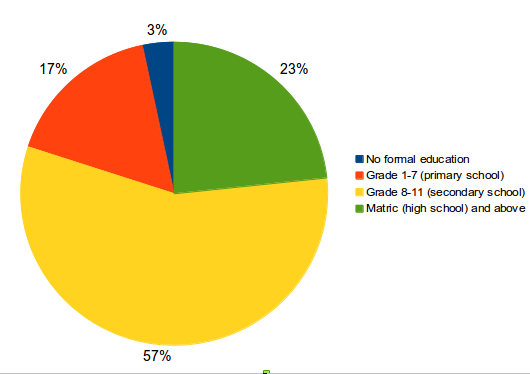
\includegraphics[width=0.6\textwidth]{Figures/education_level.png}
    \rule{35em}{0.5pt}
  \caption{Participants' income distribution.}
  \label{figure:education_level}
\end{figure}

\begin{table}[h!]
  \begin{center}
    \caption{Ethnicity of contextual inquiry's participants}
    \label{table:ethnicity}
	\begin{tabular}{|p{3cm}|p{4cm}|p{2cm}|}
		\hline
		\textbf{Ethnicity}&\textbf{No. of Participants}&\textbf{Percentage}\\
		\hline
		 Black African&8 &26.67\% \\
		\hline
		 Coloured&22& 73.33\%\\
	\hline
	\end{tabular}
  \end{center}
\end{table}

\begin{figure}[htbp]
  \centering
    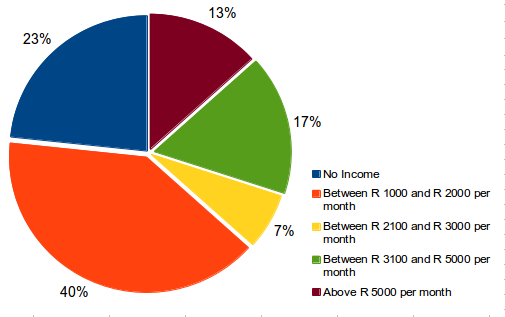
\includegraphics[width=0.6\textwidth]{Figures/income_distr.png}
    \rule{35em}{0.5pt}
  \caption{Participants' income distribution.}
  \label{figure:income_distr}
\end{figure}

Most of them participants were either overweight or obese with an average body mass index (BMI) of 33.36 kg/m\SP{2} (standard deviation of 5.74 kg/m\SP{2}). The average age was 53.13 years old (standard deviation of 11.77 years old).  Almost 86\% (26) were above 40 years of age. This means we were dealing with old participants and hence this group had a tendency of being inexperience with technology.

\section{Data Collection Methods and Analysis}
We used a semi structured questionnaire to interview participants. Each participant was interviewed for a period of 20 to 30 minutes. The questionnaire had four groups of questions and these included demographics: cellphone ownership and utilization; access to information and pedometers; and barriers to diet and physical activity. 

I used both descriptive statistics and qualitative approaches to analyse the information obtained from participants’ responses. Although our objective was to interview overweight and obese patients only but we included few participants who appeared to be thin but were diabetic. Since diabetes is a lifestyle related disease, we found that it would be interesting to also understand utilization of cellphones, and access to information even to individuals who appear not to be overweight but these individuals may had some input on various issues related technology utilization, and  barriers to behaviours that are considered healthy. All the names that are used in presentation of findings are just pseudonyms to protect privacy of participants. 
\section{Findings}
\subsection{Utilization of Cellphones}
Twenty nine out of thirty participants owned cellphones. The most used services were SMS and voice with at least 80\% of the participants using each of the two services. It was found that at least 60\% of the phones owned by participants were smart-phones (Figure \ref{figure:cell_ownership}), but utilization of functionality/services that are supported in smart-phones appeared to be lower relative to voice and SMS (Figure \ref{figure:cell_utilization}). Utilization of smart-phone supported services appeared to decrease with age. Utilization of Whatsapp appeared to be higher compared to other services that are specific to smart-phones. What led to adoption of Whatsapp is that participants were influenced by family members and friends who were already in Whatsapp. These influencers suggested Whatsapp as to be cheaper than SMS. For instance one male participant aged 47 years of age heard that Whatsapp was cheap for communication, and his son helped him on loading it into his phone. Therefore, in this context, social influence played a role in adoption of some smart-phone supported services. There is a positive correlation between social influence and adoption of high-tech innovations \citep{vannoy2010social}.  

\begin{figure}[htbp]
  \centering
    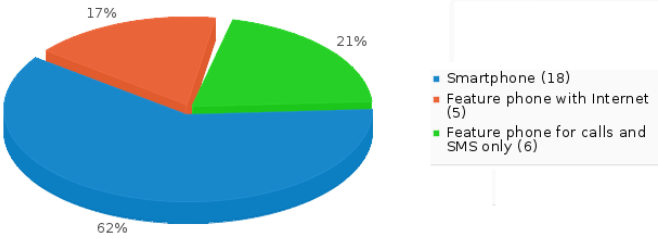
\includegraphics[width=0.5\textwidth]{Figures/cell_ownership.png}
    \rule{35em}{0.5pt}
  \caption{Participants' phones types.}
  \label{figure:cell_ownership}
\end{figure}

\begin{figure}[htbp]
  \centering
    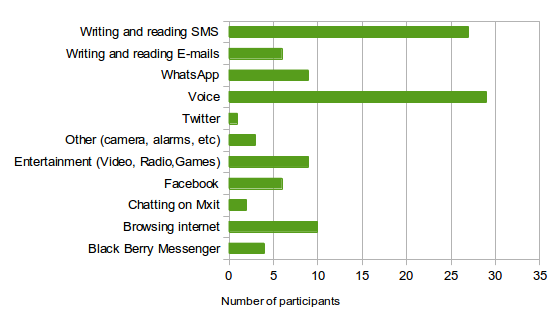
\includegraphics[width=0.5\textwidth]{Figures/cell_utilization.png}
    \rule{35em}{0.5pt}
  \caption{Participants' phones types.}
  \label{figure:cell_utilization}
\end{figure}
\subsection{Help Seeking in Utilization of Cellphones}
There were several scenarios of informal help seeking in utilization of cellphones as highlighted on Table \ref{table:intermediated}. Majority of the participants had solicited  informal help from other people before, in tasks such as: (1) to configure services/apps on their phones (e.g. Whatsapp, Facebook); (2) habituation of skills required for utilization of various functionality (e.g. a phone book of a new or unfamiliar cellphone, Whatsapp); and (3) to interact with certain features such as SMS, Internet browsers, and etc.

There was a variation in the degree of help-seeking and it was determined by how often participants wanted to execute unfamiliar tasks. Tasks such as configuration of services and apps or teaching of individuals had rare occurrences as they only happened when participants had encountered a new application or device and they don't know how to make it functional. 

\begin{table}[h!]
  \begin{center}
    \caption{Scenarios of intermediated interactions}
    \label{table:intermediated}
	\begin{tabular}{|p{1cm}|p{12cm}|}
		\hline
		 \textbf{No.}&\textbf{Scenario}\\
		\hline
		 1& She is being helped to read SMSs by her \emph{daughter}, but she could do it on her own when the daughter is not around. \\
		\hline
		2&He doesn’t know how to reply back to an SMS. So his \emph{grandson} always helps him with that.\\
	\hline
	  3&Her \emph{children} or  \emph{work colleagues} could help her to read SMS written in English that are received through her feature phone. She also mentioned that her two children were skilled in operating cellphone more than her and one of them had a Black Berry smart-phone.\\
	  \hline
	  4&He can take photos using his mobile phone’s camera but he doesn't know how to save those photos on a memory card. His \emph{son} helps him with that once in a while. But, also his son helped him in loading Whatsapp on the phone.\\
	  \hline
	  5&Her \emph{children} have taught her on how to use Whatsapp, take video etc. Now she is learning on how to record sound, set reminders on the phone for insulin and medication.\\
	 \hline
	 6&The \emph{son} would help her to interact with USSD service for checking loyalty points on MTN. MTN is a mobile communication service provider operating in many African countries.\\
	 \hline
	7&She was taught her \emph{son} on how to access a phone-book when composing SMS using her new phone.\\
	\hline
	8&She receives assistance from her \emph{helper} when she wants to send messages to her children.\\
	\hline
	9&She was once helped to do set-up her new phone at a cellphone shop. She was also taught on how to operate BBM by her \emph{grandson}.\\
	\hline
	10& He was once taught on how operate Whatsapp by his \emph{niece}.\\
	\hline
	11&Her \emph{son} and \emph{grandson} have once helped to configure Whatsapp and Facebook on her phone. They have also taught her on how to use those two web services. In addition, she also asks the son to search for certain health information on the Internet, and once the search is done the the son would pass the phone to her to view that information. This happens once in a month.\\
	\hline
	12& Her \emph{son} and \emph{grandson} always teach her on how to use various functionalities like games etc., but she is not so much keen on operating those functionalities. She also admitted that her son and grandson are so much interested with their mobile phones and they spend a lot of time playing using phones something that she doesn't understand.\\
	\hline
	13& This participant didn't own a cellphone. She had no formal education and she was unfamiliar with how to operate a cellphone. Her son receives SMS directed to her and reads it aloud for her or translates an SMS to verbal communication. Also, the son receives phone calls and hands over the phone to her when the person on the other side of the line wants to speak to her.\\
	\hline
	\end{tabular}
  \end{center}
\end{table}
\subsection{Selection of Help Givers}
Participants chose trusted individuals to act as their help givers, typically their children and grandchildren or, less often, children of relatives, family friends, or someone at a cellphone shop. Preference on who is likely to be solicited to assist favours family members. Help givers are selected based on the merit of skills/competence, and interpersonal trust based on a social relationship, and past experience of help seekers on specific help givers.
\subsubsection*{Interpersonal trust}
Interpersonal trust in this context means that whether help-seekers may feel comfortable to seek help from specific people or not. Privacy and existing relationship between a help-seeker and help-giver were first concerns when deciding of who should be asked for help. In additional to that, there was also trust on whether a helper giver may be willing to deliver when solicited for help and this was influenced by experiences in past attempts to seek help. Experiences on past attempt to solicit help refers to help-seekers' positive and negative experiences as an outcome of seeking help. These experiences shaped perceptions of some of the participants towards seeking help with cellphone or any other technology. For instance, one female participant aged 67 years old reported that her daughter helped her once but she had no patience. A male participant aged 47 years of age mentioned that he would like to be assisted on using several services such as MMS, but he thinks that young people may not be having patience to help. Such negative experiences can hinder future help-seeking behaviours from specific help givers. This resonates with the following finding by~\cite{kiesler:twi}, parents may be hesitant to seek informal help from their children after encountering negative experiences.
\subsubsection*{Help-givers' Competence}
In additional to interpersonal trust, the decision of who should be solicited for help was also influenced by help-seekers' level of trust on skills possessed by help-givers. Participants had confidence on competence of their children in using cellphones. Several participants sees their children as having technical know how skills in using cellphones. For instance one 31 years old female participant mentioned that her five years old son knows how to navigate through her whole phone and use it more than what she can do. Another female participant aged 56 years of age explained how children are eager to teach various things on a cellphone but she is not so keen in engaging to cellphones like they way her son and grandson do. A forty seven year of age male participant also mentioned that young people in their families are more skilled in cellphone than old people.
Participants reported that their kids were borrowing their phones to do other tasks and this demonstrated that their kids had better skills with technology. Scenarios of sharing are presented on Table \ref{table:phone_sharing_contextual} below. 

\begin{table}[h!]
\begin{center}
    \caption{Scenarios of sharing of cellphones between participants and their children}
    \label{table:phone_sharing_contextual}
	\begin{tabular}{|p{1cm}|p{12cm}|}
		\hline
		 \textbf{No.}&\textbf{Scenario}\\
	\hline
	1&``Zandile'', a 47 years old female participant, mentioned that her 16 years old son could borrow her phone to use MXit. But herself she is not using anything else on the phone apart from calls and SMS. She also mentioned that she is not so much interested with technology. For example she has internet at work, but she is not really using it.\\
	\hline
  2& ``Buyisiwe'', a 31 years old female participant narrated an experience about her five years old son who uses her smart-phone to listen to music. But she has to lock it while he is listening, because it happened at one point that the son deleted almost everything on the phone.\\
  \hline 
  3&``Celine', a 48 years old female participant lends her phone to her daughter who uses it for normal Internet browsing and Facebook. Celine owned an advanced feature phone enabled with Internet but she was not using internet on the phone.\\
  \hline
	\end{tabular}
  \end{center}
\end{table}
In other scenarios participants mentioned that their kids borrow their phones to search for information related to school assignments. These examples demonstrate the level of skills that potential help-givers can have. Trust on skills possessed by help-givers has been found to be very important to individuals seeking help in the ICTD and HCI contexts.~\cite{ramirez2013infomediaries} suggested that empathy and technical skills of infomediaries influence the outcomes of the process of infomediation to users at public access venues. Another study that examined motivations for informal support in utilization of computers at home found out that skills of help-givers to be one of the factors that influence help-seekers to solicit help from specific people~\citep{poole:chh}. 
\subsection{Access to Health Information and Self-Monitoring Support}
We have collected information about access to health information and self-monitoring support among our participants.The information support in which most the participants relied on is that one provided through face to face meetings with doctors or dieticians during hospital visits. Normal hospital visits are scheduled in intervals of every 3 or six months. But they do visit the hospital only two or three times in a year. In addition to face to face information, patients normally receive paper sheets with information that provide guidance on how to eat healthy. These paper sheets are normally received when patients attend clinic for the first time after being diagnosed with diabetes. Most patients we interviewed were type 2 diabetic and overweight. Doctors and nurses encourage them to eat healthy and exercise. 

Majority of the participant lacked informational support beyond hospital settings that can provide guidance in eating healthy and exercising. Very few participants had used cellphone services as means of querying or receiving information related to health. Only six participant had used internet to search for health information, while only one participant had used a cellphone app for health. Also only two participants had used SMS while only one had used voice to look for health information. Table shows some of the scenarios of where participants had used ICTs in relation to learning about issues concerning their health.
\begin{table}[h!]
\begin{center}
    \caption{Participants’ usage of ICT to fullfil health information needs}
    \label{table:health_information}
	\begin{tabular}{|p{1cm}|p{12cm}|}
		\hline
		 \textbf{No.}&\textbf{Scenario}\\
		 \hline
		 1&``Anitha'', a female participant aged 56 years old, would send SMSs to her son while he is at his workplace. This SMS is usually a request to check for certain  health information on the internet and the son could print for all the material related to that information that was requested. She also follows Dr Oz program on TV about health stuff. If she misses she would go to the Internet and visit the programme's website\\
	  \hline
	  3& ``Jane'', a female participant aged 36 years old, had an app on her phone for giving health tips. She downloaded that app from the Internet.\\
	  \hline
	  4& ``Maria'', a female participant aged 57 years old mentioned that she uses Facebook. She has three diabetic friends and they share diet concerns, recipes, and discuss diabetic specific issues that they experience . They don't discuss about exercise. She sometimes searches on Google about medications especially when she starts using new medications. She uses Google to get more information on the things her doctor advises on.\\
	  \hline
	  5& ``Evelyn'', a female participant aged 63 years old, subscribes to health websites to receive emails with health tips and information. She sometimes calls a dietician to ask about certain diet information.\\
	  \hline
	\end{tabular}
  \end{center}
\end{table}

Self-monitoring of blood glucose seemed to be common among the participants because many of them were diabetic. Self-monitoring of other health parameters such as diet and physical activity seemed not to be done by many participants. Out of thirty participants we interviewed, only two participants had used a pedometer before.  One participant reportedly to use a gym bicycle with a meter that can show distance cycled but she has abandoned using it. Only eight participants reported that they have used a diary before to record the food they have eaten. But this recording is not consistent. Some have stopped doing it although they claim that when they visit hospital, sisters (nurses) always remind them to record foods they have eaten. This food recording is mainly for controlling the levels of blood glucose. For instance, one participant mentioned that she has a note of where she records the blood glucose before she eats and the blood glucose after she has eaten. So she records what she has eaten and the blood glucose levels before and after meals. But overweight and obese diabetic patients are also encouraged to lose weight. Because losing weight has an advantage of lowering levels of blood glucose.  And the only way to lose weight is to follow the recommended diet and become more physically active. 
\subsection{Barriers to Adoption of Healthy Behaviours}
The research teams also examined on barriers to adoption of healthy behaviours such as healthy diet and exercises.

On barriers towards adoption of healthy diet, 76\% of the participants mentioned that the recommended healthy food is always expensive. For instance fat free foods are much more expensive compared to full fat foods. One participant associated eating of certain food cultural upbringing. She explained that Muslims in Cape Town often have very high fat and high sugar content foods  such samosas. One of the comments that appeared to be common to many participants is that; it is difficult to have a budget for separate meals within the family, because diabetic members always have their diet food which seems not be preferred by the rest of the family. So diabetic members might end up eating what the rest of the family eats. They do try to have diet foods by it is not always manageable. But one participant who seemed to be highly motivated disagreed with that argument and said most people lack an understanding of what carbohydrate means. She further mentioned that, education about diet should be contextualized to terms that people are already familiar with. She said most people don't understand what is said by dieticians because it is not communicated in the context they understand. For example the concept of carbohydrates is not well comprehended by many people. But if the topic is well explained using what is already familiar to patients, then they are more likely to comprehend it.

On the question of perceived barriers to physical activity, nine(9) participants mentioned that lack of time to do physical activity because of a busy schedule contributes to less exercising. This is supported by some remarks shared by participants on Table \ref{table:busy_schedules}. Seven participants mentioned that lack of areas to walk around is one of the perceived barriers to physical activity. The most common comment given out to support this argument was that, most of the areas where they live are not safe for somebody to be out walking all the time (Table \ref{table:safety_issues}). Most of these areas have high rates of crime.

\begin{table}[h!]
\begin{center}
    \caption{Excerpts on observation of common participants’ remarks on association between being less active and busy schedules}
    \label{table:busy_schedules}
	\begin{tabular}{|p{2.5cm}|p{10.5cm}|}
		\hline
		 \textbf{Participants}&\textbf{Remarks}\\
	  \hline
	  1&She goes to work very early in the morning and comeback late at night.\\
	  \hline
	  2&Difficult to manage work and household.\\
	  \hline
	  3&She goes to work at 4.00 AM and come back at 7.00 PM. She works for 6 days in a week.\\
	  \hline
	  4&She looks after the family. She takes her sisters child to school, also she does the cooking. She does a lot of house work. So it is difficult to have a planned series of physical activity.\\
	  \hline
	 5&Difficult to balance between planned session for physical activity and manage both work and household at the same time.\\
	 \hline
	 6&Busy with house work at home.\\
	 \hline
	\end{tabular}
  \end{center}
\end{table}

\begin{table}[h!]
\begin{center}
    \caption{Excerpts on observation of participants’ remarks on safety concerns on areas to do walking or running}
    \label{table:safety_issues}
	\begin{tabular}{|p{2.5cm}|p{10.5cm}|}
		\hline
		 \textbf{Participants}&\textbf{Remarks}\\
	  \hline
	  1&The neighbourhood is not safe to wonder around.\\
	  \hline
	  2&It is not safe in her area. She doesn't like to be outside most of the time.\\
	  \hline
	  3&It is unsafe at night and early morning.\\
	  \hline
	  4&The area where she stays is not safe to walk around.\\
	  \hline
	 5&Not safe to walk alone. She prefers to walk through houses.\\
	 \hline
	\end{tabular}
  \end{center}
\end{table}

But despite the claim of lack of both time and areas to exercise these participants mentioned that they been active when doing their daily errands (Table \ref{table:daily_activity}). 

\begin{table}[h!]
\begin{center}
    \caption{Excerpts on observation of participants' remarks regarding physical activities that were part of their daily lives' routines}
    \label{table:daily_activity}
	\begin{tabular}{|p{2.5cm}|p{10.5cm}|}
		\hline
		 \textbf{Participants}&\textbf{Remarks}\\
	  \hline
	  1& She walks from home to visit relatives and friends.\\
	  \hline
	  2&He only walks when he goes to church.\\
	  \hline
	  3&She walks to from her home to a bus station everyday and walks a lot at her work place, so it would be great for her to have something to keep track of how much exercise she gets. She wants to be more active but works 7 days a week.\\
	  \hline
	  4&She exercises in a group of people for three times a week and she now feels much healthier. They have a "biggest loser" competition going at the moment. She would like to have a pedometer to keep a better track of her activity.\\
	  \hline
	 5&She only walks when she has to. She only walks up and down in kitchen. She has a treadmill, but she doesn't use it.\\
	 \hline
	\end{tabular}
  \end{center}
\end{table}

\section{Contextual Design Insights}
There has been an advocacy of moving management of lifestyle related chronic conditions from healthcare system to citizen-centric health promotion and disease prevention interventions \citep{korhonen2010personal}. Advancement in hardware and software technologies has enhanced automation of health self-management processes \citep{arsand:mobile}. Health self-management programs usually ask their participants to keep records of their activities, physiological variables and other health-related data; and ICT systems such as personal informatics applications can make this process simpler and easier \citep{medynskiy2010salud}. In this context, majority of the participants were not utilizing ICTs in self-management of their healthy as they relied on paper diaries. The only parameter that was being monitored by majority of the participants was blood glucose since all participants were diabetic. Blood glucose is usually controlled through many factors such as diet, exercise, and medication. Type 2 diabetes is linked to obesity and its self-management is mostly through diet and exercise.  The process of self-management can be very cumbersome if it is done using pen and paper and this may reduce compliance \citep{mattila2008mobile}. A paper diary may not be as effective as an electronic diary when it comes into navigating across behaviour patterns for the purpose of self-reflection. Therefore, personal health apps may be important in supporting self-management of health. However, these personal health apps may not be very useful in this context considering the fact that majority of the participants have limited skills in operating technology. The findings above indicate that some participants with limited skills seek help from people with skills. But this approach has its limitations as it relies on existing intrinsic motivation of help givers. Long term usage is crucial for compliance \citep{mattila2008mobile}, but one cannot achieve this long term usage in the context where a technology needs to be utilized through help givers while most technologies were not designed to anticipate utilization through help givers as part of the usage ecosystem.

Sharing of phones between adults and kids suggests that it is feasible to design a system of which both kids and parents can have access to. What was observed from above is that kids borrow phones because they are motivated with specific things on the phone. One of those things is social media. Therefore if one could design a system that afford specific motivational needs of kids and integrate it with self-monitoring of behaviours of adults then we can enhance motivation kids to help their parents with self-monitoring tasks. In the next chapter, I discuss about the theoretical framing in designing a system that could motivate kids to assist their parents in self-monitoring tasks.

\begin{flushright}
\end{flushright}
% Chapter 1

\chapter{Prototype I} % Main chapter title

\label{prototype1chapter} % For referencing the chapter elsewhere, use \ref{Chapter1} 

\lhead{Chapter 1. \emph{Prototype I}} % This is for the header on each page - perhaps a shortened title
%----------------------------------------------------------------------------------------
\section{Development of the Prototype}
In this phase, I developed the first version of the application prototype. The prototype had features that allow individuals to self-monitor activity and diet.  The manipulation of user interfaces of the app was specifically targeted to help givers/intermediary users. The prototype was designed to encourage a help-giver and a help-seeker to work together in a pair. To make the act of helping to be perceived as more meaningful, the first message on the app emphasized that the intermediary users were helping someone close to them to manage their wellness.  To motivate ongoing use, the app had gamification features of where each pair could be awarded points, badges, nice looking gardens and fish tanks. In additional, within each pair's garden and fish tank, there was a Facebook social plug-in that could allow users from different teams/pairs to comment on or like each other. We also utilized Facebook groups to remind users to engage with the application. Ideally, the information flow supposed to be as suggested on Figure \ref{figure:prototype_1}. A web app was developed using a combination of several web technologies such as HTML, JQuery, JavaScript, and CSS on the client side, while the server was implemented using Django Python framework. Sample screen-shots of the prototype are shown on Figure \ref{figure:prototype_1_screens}. Authentication was done through Facebook accounts of intermediary users''. This prototype aimed at encouraging increase in physical activity and  decrease of sedentary behaviours through informing individuals (help-seekers) about their level that could have an impact on their health. In addition, also individuals could monitor whether they are eating healthy or not. Some visualization techniques that are similar to this have been previously used  in systems that were designed for direct users such as ``Fish'n'Steps''\citep{lin2006:fish}, ``Ubifit''\citep{klasnja2009:using},  and ``Few Touch Application''\citep{arsand:mobile}. The idea of using a plate for showing distribution of meals is mimicking a practice used by dietitians of where the amount of each food group that needs to be consumed is presented as a bisector of a pie chart. 
   
\begin{figure}[htbp]
  \centering
    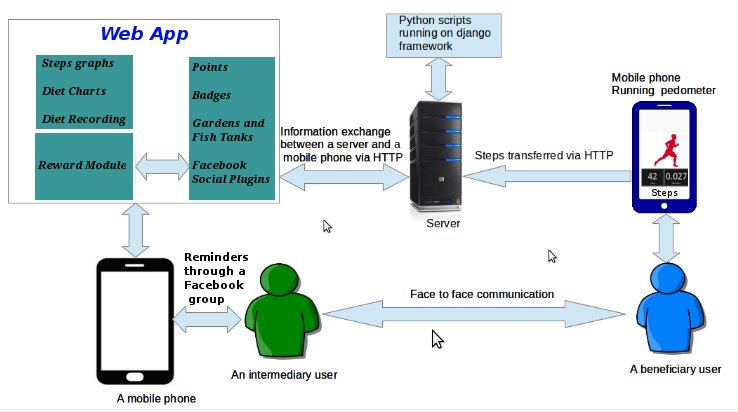
\includegraphics[width=0.8\textwidth]{Figures/prototype_1.png}
    \rule{35em}{0.5pt}
  \caption{Information flow in the first prototype.}
  \label{figure:prototype_1}
\end{figure}

\begin{figure}[htbp]
  \centering
    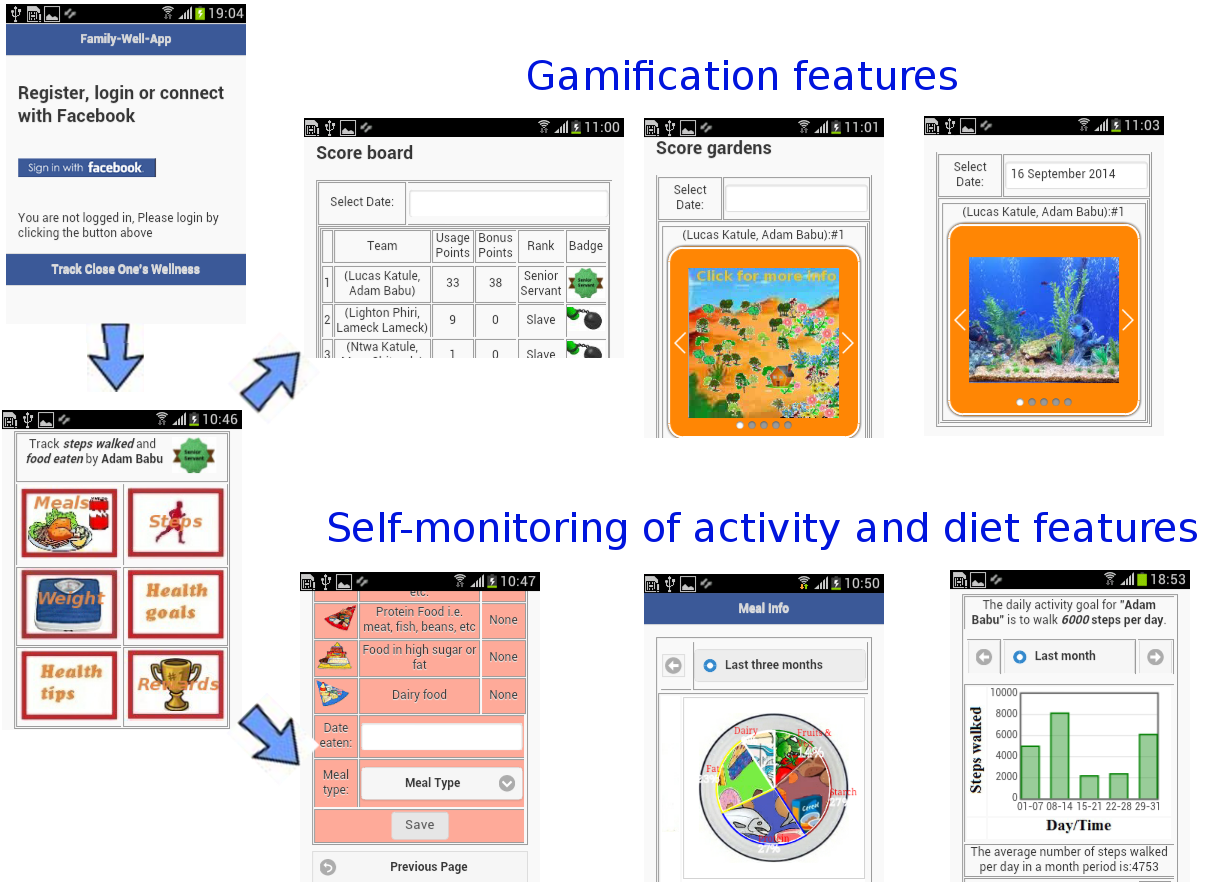
\includegraphics[width=0.8\textwidth]{Figures/Version1/Prototype1Screenshots.png}
    \rule{35em}{0.5pt}
  \caption{Sample screen-shots of the first prototype}
  \label{figure:prototype_1_screens}
\end{figure}
\section{Prototype Evaluation}
In order to evaluate the prototype, I recruited participants through an NGO
based in Cape Town called ``\textbf{\textit{Mamelani Projects}}''. This NGO
carries out outreach programs on health education in less privileged
communities. Mamelani trains women onissues of HIV/AIDS, nutrition, and gender equality. 

The NGO helped to recruit participants among people who were part of their trainings in Philippi township. Criteria for recruitment were as follows: (1) participants aged 35 or above and (2) participants must have an intermediary person willing to work with them. The NGO identified the targeted participants that met the inclusion criteria. A total of six adult participants were recruited of which both were women above middle age (\textgreater= 35 years of age). Each one of the adults brought one intermediary to form a pair. Three intermediaries were girls in between 19-23 years of age. The remaining three intermediaries were boys aged between 14 and 19 years of age. 

Participants were informed of their rights . Participants were also informed of which of their information will be collected by the study. Both adults and their respective intermediaries signed consent forms except for intermediaries who were minors, these signed assent forms that were approved by their respective parents/guardians. 

The next step entailed training of intermediaries on how to use the app. The application was deployed to the field from the end of October 2014 to beginning of December 2014. In order to control the application environment, and limit potential complications from deploying the intervention on multiple platforms, each pair of participants was given one Android phone (Samsung GT-S5300) running the pedometer app. Participants were required to utilize the web application hosted at University of Cape Town by using a web browser built into their phones. In order to retain participants in the study each intermediary participant and each beneficiary participant who remained as part of the study received ZAR30 (\~US\$3) worth of airtime every week for the duration of the study. I collected qualitative feedback in the middle and at the end of the study
\section{Findings}
Observations and qualitative feedbacks from the six cases/pairs are presented below. The first three pairs consisted of parents working their children while the remaining three pairs it was just an adult working with either a close or distant relative in each pair.
\subsection*{\textbf{Pair 1: Mother and Son}}
This pair consisted of a boy aged 17 years of age working with his mother. The boy is referred here with the name ``\textbf{Jabulani}'' and his mother is referred with the name ``\textbf{Nandipha}''. Jabulani lives with his mother and other siblings. He seems to be passionate with social networks. He currently uses Twitter, and Facebook mostly. He mentioned that he felt happy helping his mother. He also articulated the reason for helping his mother as that he felt it was his duty since the mother took care of him when he was growing up. Nandipha also felt very happy being helped by her son and she mentioned that she thinks her son is very brilliant more than her and she gets to know things because of him. 

Jabulani acted as an intermediary for his mother. He was the first one to engage with the app for at least three different days. All of a sudden his use stopped. When I asked Jabulani together with his mother of challenges that might have prevented them from using the app, their responses indicated that were more conscious about airtime as it was one of the reasons of why they didn't  login more often. So there were times where they ran out of time. They thought having more data bundles might solve the problem. Another reason for why they didn't use the app more often is associated with lack of competitions from other pairs and also they had accomplished the highest challenge within few days. In the first few days they were so curious about attaining the highest badge. Jabulani claimed that her mother was walking up and down so that they reach that goal. Jabulani discussed with his mother that they must reach that goal in  a week. They managed to reach the goal and there was no more boundary to break.

Badges were one source of motivation to this pair. Jabulani felt motivated by the badges and he was persuading his mother to work harder so that they reach the highest badge which was Queen/King. Also, Jabulani noticed something on the scoreboard. He and his mother were there leading. Another team (Pair 3) was in the second position. The third position was held by Pair 4. Then after few days Jabulani noticed that Pair 4 moved from a third position to a second position. So Jabulani told his mother that ``we must not drop down because Pair 4 is going to reach us. So competition with others was a source of motivation for Jabulani. Although Jabulani was helping his mother but he thought like the ownership of the winning process as theirs because he used the word “We” all the time to imply that he felt that he was part of that process. Additionally, Jabulani liked information displayed by a botanical garden and a fish bowl. He expalned why he was so interested in such abstract visualizations. When he was growing up he used to watch cartoons. So when he sees those pictures of trees and fish he feels he is part of that process of making those images/cartoons. So drawing fish and trees through their team's performance motivates him more and he tells his mother that they must have more fish in the bowl. Also the idea of fish in the bowl motivated Nandipha. She mentioned  that she doesn't like to see her bowl empty without any fish, so she tries to walk more steps as she can. These ideas of abstract visualization such as fish bowls/tanks and garden have been previously used in system that involve only one user on interaction with user interfaces \citep{lin2006:fish, klasnja2009:using}, the only difference in this context is that, the same ideas were extended and tested with two users who are collaborating to attain one objective. 
\subsection*{\textbf{Pair 2: Mother and Son}}
``\textbf{Dumisani}'' was a 14 years old boy who lived with his mother, ``\textbf{Kholiwe}''. Dumisani was acting as an intermediary for Kholiwe. Dumisani and Kholiwe used the system for only the first three days and they dropped out. On responding to the question of why was it the case, Kholiwe mentioned that it was the inability to access the system every time they tried out. The web page was always giving them time-outs and this discourages them from trying. But it was also observed that Dumisani was not very familiar with Facebook authentication as he didn't have an account before. I created one account for him of which it wasn't very helpful. The decision in using Facebook authentication was based on an assumption that all intermediaries may have Facebook accounts which was no the case. However, despite technical challenges this pair also showed enthusiasm in using the app.
\subsection*{\textbf{Pair 3: Mother and Daughter}}
``\textbf{Zama}'' was a 20 years old girl who was supposed to act as intermediary for her mother, ``\textbf{Fikile}''.  Since the daughter appeared to be interested to help her mother, then one would think that intermediation is possible. Unfortunately, the two lived in different houses and they never used the system at all. Their contact to discuss issues about the system was limited as Zama was raising a toddler at that time. In addition, Fikile appeared to had some expertise in using technology as she already was using Facebook, therefore she was interested to learn how to operate the system on her own because of the situation of her daughter. However, the system had been set up only to allow Facebook account for Zama. 
\subsection*{\textbf{Pair 4: Close Relatives}}
``\textbf{Lindiwe}'' is a young girl in her early twenties. Lindiwe was acting as an intermediary for her auntie ``\textbf{Nceba}'' but they never lived together in the same house. The pair had not been interacting with the application at all. When I interviewed Nceba of why they were not using the app,  her response was that she doesn't know how to operate it on her own and her intermediary seems not  to be around most of the time. She is curious to access the information but her intermediary seemed not to be cooperative. So she suggested to bring someone else who was also a close relative.
\subsection*{\textbf{Pair 5: Close Relatives}}
``\textbf{Neliswa}'' was a girl aged 23 years of age. Neliswa  was acting as an intermediary for her auntie ``\textbf{Nkosazana}'' but they lived lived together in the same house. The pair had not been interacting with the application at all. I never had a chance to interact with this pair since they were not available. But from a personal observation during recruitment, Neliswa appeared to be less interested in the intervention even though he signed the consent form to participate. 
\subsection*{\textbf{Pair 6: Distant Relatives}}
``\textbf{Nkululeko}'' was a boy aged 19 years of age. He was acting as an intermediary for her distant relative, ``\textbf{Noluthando}. Nkululeko and Noluthando didn't live so close to each other but they did see each other more often. System logs showed that this team had not been engaging with the application. I interviewed both of them to find why that was the case. Nkululeko pointed out number of things. The first one was that he tried to access the application a couple of times but he was unable to proceed after login. He was using his personal phone. I checked his personal phone and I discovered that his web browser was the problem. He had never tried to do it using the experimental phone that was in possession of Noluthando. He had ne We tried together and it was okay on the other phone.  But in addition to phone's problems he claimed to be busy with school. Despite him being busy, and his phone not being able to support the application,  the absence of things like reciprocal benefits  and a close social relationship with the beneficiary, might be the cause for his low intrinsic motivation in engaging. The previous user, Jabulani had a problem of accessing the application using his personal phone but he made an effort to access using the phone  given to his mother. So the closeness/bond of the two sets users might be the base for the network effect to happen.
\subsection{Discussion}
Only two pairs of users engaged with the system for more than two days. Both of these two pairs consisted of a beneficiary and an  intermediary living in the same house. These pairs consisted of mothers working with their sons. One of these two pairs was very motivated and enthusiastic about the system. But after some time they also got bored because they were not getting any competition from other teams and they had attained all the challenges within a short period of time. In a third pair, a girl was working with her mother but they were not living together so it was difficult for her to commit to the application. Intermediaries from the remaining two pairs showed little enthusiasm in the project. There were three hypotheses for this lack of enthusiasm to engage with the system and these were: (1) due to lack of motivation to engage with system; (2) lack of a prior social relationship between the two users within each pair; and (3) Low frequency of interactions between the two users within a pair due to distance.

There was an indication that a prior social relationship is instrumental for intermediaries to perceive value in the act of helping their beneficiary users. In this case the interaction became more meaningful. It also becomes easier for the two users within a pair to negotiate for interaction. For three pairs that consisted of mother/son or mother/daughter there was a tendency for the two users to show the eagerness of working together. For three pairs where members of a pair didn't  have a parent/child relationship, intermediaries showed little enthusiasms in the intervention. Another advantage of a prior social relationship comes to sharing of phones. It was observed that it was easier for an experimental phone to move from a beneficiary to an intermediary when a parent and child were involved in a pair. There was a form of trust that existed between the two users with a prior social relationship. In addition, intermediaries had more authority when they were helping a person who was close to them. If a pair with a prior social relationship needed to interact with the app, then the frequency of these interactions depended on proximity between the two users. For cases where they cohabited or lived nearby it increased the chances of them meeting. For instance, ``\textbf{Zama}'', an intermediary participant aged 20 years old was working with her mother. The challenge with this pair is that they didn't cohabit and Zama had a toddler hence this lowered her ability to participate in the intervention.  

Prior social relationship also worked in parallel with the presence of interest to use the app/gamified features. A combination two factors played a some role in  encouraging the two users within a pair to collaborate when they met. For instance , in the case of of Jabulani and Nandipha (mother and son), they discussed about strategies to win against other pairs. Although Jabulani was helping his mother but he thought like the ownership of the winning process is theirs because he used the word ``We'' all the time to imply that he felt that he was part of that process. In addition, if intermediaries are motivated they can become persuaders of beneficiaries that they have a prior social relationship with as it can be seen on Jabulani who encouraged his mother to walk more steps.

There were some drawbacks in utilization of this prototype. From participants' perspective , intermittent internet connectivity, insufficient airtime, less motivated intermediaries, and lack of competition/challenges with others in the gamified system were the key issues mentioned. Other factors include how often the two user meet (Whether they cohabit or they meet more often), and reminders were not timely. I had very high expectations that Facebook reminders will work for this community. An assumption was that every intermediary is probably using Facebook. Actually this was not the case. There were some intermediaries who had never engaged with Facebook before. And the ones who had engaged with Facebook were not doing it so often as I anticipated. For instance ``Jabulani'' had never used Facebook before. ``Jabulani'' was only engaging with Facebook at most twice in a week. Therefore, Facebook might not be an on time-platform for delivery of reminders or any messages to intermediaries in this context.  

Findings from this informative evaluation led to another iteration in the design. It also informed the manner in which evaluations in chapters \ref{prototytpe2chapter} and \ref{summativeevalchapter} were conducted.
\begin{flushright}
\end{flushright}

% Chapter 1

\chapter{Prototype II} % Main chapter title

\label{prototytpe2chapter} % For referencing the chapter elsewhere, use \ref{Chapter1} 

\lhead{Chapter 1. \emph{Prototype II}} % This is for the header on each page - perhaps a shortened title

%----------------------------------------------------------------------------------------
\section{Prototype Development Iteration II}
\section{Prototype Evaluation Description}
\begin{itemize}
\item{Location}:
\item{Recruitment of Participants}:
\item{Participants Demography}
\end{itemize}
\section{Prototype Evaluation Methods}
\section{Findings}
\begin{flushright}
\end{flushright}

% Chapter 1

\chapter{Summative Evaluation} % Main chapter title

\label{summativeevalchapter} % For referencing the chapter elsewhere, use \ref{Chapter1} 

\lhead{Chapter \ref{summativeevalchapter}. \emph{Summative Evaluation}} % This is for the header on each page - perhaps a shortened title

%----------------------------------------------------------------------------------------
\section{Recruitment of Participants}
With help of a research assistant who was a resident of Langa,  we managed to recruit a total of fourteen adult participants (beneficiary users). We recruited these participants from two townships in Cape Town: Langa, and Athlone. In Langa there were five adult participants while in Athlone there were nine adult participants. The average age of these adult participants was 44.21 years with a standard deviation (S.D) of 9.99 years. The youngest adult was 26 years of age while the oldest was 60 years of age. Thirteen participants were females. 

Each adult participant (beneficiary user) elected one of their children/grand children to become their intermediary user to form a pair of users. The two members of a pair were required to work together in using the ``Family Wellness App'' to self-monitor the wellness of one member of a pair (a beneficiary user). All beneficiary users were working with their children but one whom was was working with her grand child.  The average age of children participants (intermediary users) was 15.42 (S.D=2.06) years. The youngest intermediary user was 12 years of age while the oldest was 20 years of age. The number of females and males intermediary users were equal. 

I gave detailed information of what the study was all about to both intermediary and beneficiary participants. I informed them about different modes of which I will collect data. All beneficiary participants signed informed consent forms agreeing to be part of the study. Since all intermediaries were under 21 years of age, they signed assent forms which were also signed by their parents/guardians who were part of the study.

I allocated one day to teach intermediary participants on how to use the ``Family Wellness App''. In addition, each intermediary was given a user manual. After the training, I gave out one Android phone (Samsung GT-S5300) to each pair of participants. These phones were installed with two natives apps. The first app was a pedometer and the second one was the main ``Family Wellness App''. The ``Family Wellness App'' loaded all its content from a web application hosted remotely. The app was used for a total period of six weeks. Each pair of participants provided the service provider's number of the SIM card that was inserted on their given Android phone. I allocated 1.3 GB of data to each SIM card. In addition each beneficiary participant was given a total of ZAR 240 as a compensation for transport and their time for the duration of the study. The details of the experiments are outlined on the next section.

\section{Experiments}
This phase of the study evaluated the effectiveness of gamification/rewards in motivating both intermediaries and beneficiaries to engage with the ``Family Wellness App''. I was comparing two versions of the applications. The first version of the application was simply a logbook or journal that allows each pair of users to record and view wellness data of a beneficiary member of the pair. With the logbook app users could view physical activity feedbacks and recording and viewing summaries of nutrition components of food consumed by a beneficiary within a pair. The second version of the application was an extension of logbook to include rewards/gamified subsystem. I carried out this evaluation for a period of six weeks. I carried out the experiments from the mid-October 2015 to the end of November 2015.  The details of how experiments were designed and how data were collected are presented on the next sub-sections.
\subsection{Experiment Design}
I used ``within-group'' design for the experiments. In within-group design, the same group of participants is exposed to different experimental conditions. This helps to minimize the number of groups needed to test hypotheses as only one group is used for both control and intervention. Another advantage of within-group design is that it minimizes the effect of confounding factors. The only problem with this approach is the learning effect and it lengthens the duration of the study. In order to minimize the impact of the learning effect on the outcome, I randomly assigned pairs of participants to two separate groups referred to as experimental sequences. The first experimental sequence started with the ``Logbook App''  and finished with the ``Gamified App''. The second experimental sequence started with the ``Gamified App'' and finished with the ``Logbook App''. I used the following abbreviations ``LG'' and ``GL'' to refer to the first and second experimental sequences respectively.

A total of seven pairs of participants were assigned to the LG group while the remaining seven pairs were assigned to the GL group. Both groups spent the first four weeks in their first experimental conditions of which the Logbook App for the LG group and the Gamified App for the GL group. After 27 days each group was switched to a different experimental condition. The LG group started using the Gamified App while the GL group started using the Logbook App. The second phase of the experiment lasted for a total of 14 days. In the next sub-section, I provide details of how data were collected during the duration of 41 days (6 weeks) of running the experiments. 

\subsection{Data Collection Methods}
Data collection was a triangulation of application's logs,questionnaires and interviews. 
\subsubsection{Family Wellness App Logs}
Application's logs consisted of information regarding the time when there were users' activities on the app, the pair that was accessing the app at that time, and the functionality that was being accessed by that pair. Logs were categorized to their respective experimental condition. 
\subsubsection{Questionnaires}\label{methodsquestionnaire}
I administered questionnaires at the baseline, mid-line (during switching of experimental conditions), and end-line. The list of questionnaires is provided below.

\textbf{Baseline Questionnaires}

At baseline both intermediary and beneficiary participants filled their respective questionnaires. 
\begin{itemize}
\item{\textbf{Intermediaries}}: Intermediaries participants' baseline questionnaire had three sections. The first section captured demographic information such as age,gender, and number services/apps used on cellphones. The second section included an IMI (Intrinsic Motivation Inventory) questionnaire  to assess participants' intrinsic motivation in using cellphones. The third section included an IMI questionnaire to assess participants' intrinsic motivation in helping their parents with cellphone based tasks.
\item{\textbf{Beneficiaries}}: Beneficiary participants' baseline questionnaire had four sections. The first section captured demographic information such as age,gender, and number services/apps used on cellphones. The second section included an IMI questionnaire to assess participants' intrinsic motivation in using cellphones. The third section included an IMI questionnaire to assess participants' intrinsic motivation in self-monitoring of diet/nutrition.The fourth section included an IMI questionnaire to assess participants' intrinsic motivation in self-monitoring of physical activity.
\end{itemize}
\textbf{Midline Questionnaires}
Also at midline both intermediary and beneficiary participants filled their respective questionnaires. 
\begin{itemize}
\item{\textbf{Intermediaries}}: Intermediaries participants' midline questionnaire had only one section which included an IMI questionnaire  to assess participants' intrinsic motivation in using the family wellness app.
\item{\textbf{Beneficiaries}}: Beneficiary participants' baseline questionnaire had four sections. The first section included an IMI questionnaire  to assess participants' intrinsic motivation in using the family wellness app. The third section included an IMI questionnaire to assess participants' intrinsic motivation in self-monitoring of diet/nutrition.The third section included an IMI questionnaire to assess participants' intrinsic motivation in self-monitoring of physical activity.
\end{itemize}

\textbf{Endline Questionnaires}
At endline both intermediary and beneficiary participants filled their respective questionnaires. 
\begin{itemize}
\item{\textbf{Intermediaries}}: Intermediaries participants' endline questionnaire had only one section which included an IMI questionnaire  to assess participants' intrinsic motivation in using the family wellness app.
\item{\textbf{Beneficiaries}}: Beneficiary participants' endline questionnaire had three sections. The first section included an IMI questionnaire  to assess participants' intrinsic motivation in using the family wellness app. The third section included an IMI questionnaire to assess participants' intrinsic motivation in self-monitoring of diet/nutrition.The third section included an IMI questionnaire to assess participants' intrinsic motivation in self-monitoring of physical activity.
\end{itemize}

I developed the IMI questionnaires with guidance of materials found on a ``Self-Determination Theory''\footnote{http://www.selfdeterminationtheory.org/intrinsic-motivation-inventory/} website which is maintained by researchers working on the theory including Richard Ryan and Edward Deci\citep{deci1985intrinsic} whom were early pioneers in developing the theory. I pretested these questionnaires during the informative evaluation of prototype II in chapter \ref{prototytpe2chapter}.  The most most important sub-scales for our theoretical construct were perceived competence and perceived autonomy which are part of the three basic psychological needs. The relatedness sub-scale is not yet validated but it was included in all questionnaires. Other sub-scale that was included in all questionnaires is perceived enjoyment. In each question from the IMI sub scales, respondents were supposed to rate there experience in a scale of 1 to 7 points which means that 1 implies the statement is "not true at all" and 7 means the statement is "very true". \newline
Perceived enjoyment is the only direct measure of intrinsic motivation while perceived competence and perceived autonomy are predictors of intrinsic motivation. Self-Determination theory suggests that a behaviour can be started as externally motivated and if external motivators support the three basic psychological needs which are relatedness, competitiveness, and autonomy then a behaviour that was once externally motivated can be internalized and users will start doing it because it is a good thing to do.

\subsubsection{Interviews}
I also conducted short unstructured interviews at midline and endline. I selected fewer intermediaries and beneficiaries for the interviews. Interviews responses were important in supplementing data collected through questionnaires and application's logs.
\section{Findings}
There were four primary outcomes in analysing the findings and these are: (1)usage trend of the app; (2) user experience/intrinsic motivation  of both intermediaries and intermediaries in using the app; (3) intrinsic motivation of beneficiaries in self-monitoring of diet/nutrition; and (4) intrinsic motivation of beneficiaries in self-monitoring of physical activity.
\subsection{Analysis of Usage Trend}
The average number of days on which pairs used both versions of the application was 10.5 (SD=7.39) days. The most active usage was from a pair that utilized the app for a total of 26 days. The less active usage was from a pair that had used the app for only two days out of 41 days.\newline
I contrasted usage in each day between the ``Logbook App'' and ``Gamified App'' by computing the daily total number of sessions from all users in each of the two experimental conditions. The beginning of a new session is defined as the a continuous period of time where the end user interacts with the app without interruption. This period is whereby there is user's activities detected on the app while there was no user activities for the past one hour. If delay between activities is less than one hour it is then assumed that the last session is still active. If a user comes back after one hour has elapsed since the last detected user's activity then it is assumed they went away from the app and now they are coming back for a new session. There were 41 days of app usage in total. Therefore, each experimental condition had a total number of sessions for each day as shown on Figure \ref{figure:usagedailysessions}. After the fourth week there was a decline in the daily total number of sessions in each of the two experimental conditions as the result of the learning effect. The decline was more apparent to users who where switched from gamification to logbook since the switching happened at the end of the fourth week of usage.\newline
\begin{figure}[htbp]
  \centering
    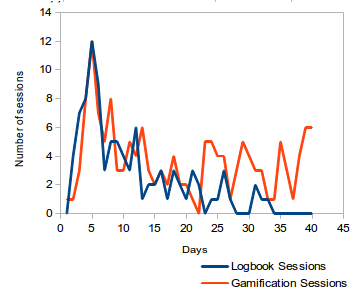
\includegraphics[width=0.6\textwidth]{Figures/scatter_daily_sessions.png}
    \rule{35em}{0.5pt}
  \caption{Total daily number of sessions from the two experimental conditions.}
  \label{figure:usagedailysessions}
\end{figure}\newline
I expanded the comparison of Figure \ref {figure:usagedailysessions} by carrying out an inferential statistical test in order to determine if the daily total of number of sessions differs in between logbook and gamification conditions. Before deciding on which test to use, I applied``\emph{Shapiro-Wilk Normality Test}''\footnote{http://sdittami.altervista.org/shapirotest/ShapiroTest.html} to test for normal distribution in both daily logbook and gamification sessions. The distributions of the two independent samples were both not normal. An attempt to transform the data using transformation algorithms didn't yield to normal distributions. Therefore, I made a decision to use a non-parametric test called Mann-Whitney U Test. The  daily number of sessions in gamification condition were significantly higher than in logbook condition as shown on Table \ref{table:usagedays}.
\begin{table}[h!]
  \begin{center}
    \caption{Daily usage comparison between Logbook and Gamified systems for 41 days}
    \label{table:usagedays}
	\begin{tabular}{|L{3cm}|c|c|c|c|c|c|}
		\hline
		Groups&N&Rank Average&Sum Ranks&U&Z&P\\
		\hline
   		Daily logbook sessions&41&33.72&1701.5&\multirow{2}{*}{1159.5}&\multirow{2}{*}{-2.9538}& \multirow{2}{*}{0.00318}\\\cline{1-4} 
   		 		    Daily gamification sessions&41&49.28& 1701.5&&&\\
\hline
	\end{tabular}
  \end{center}
\end{table}
I conducted another usage comparison which  entailed contrasting `Logbook'' usage versus ``Gamification'' usage for each pair as the aforementioned analyses were general not specifically examining on the performance of individual pairs and its results are shown on Table \ref{table:usagewellness1}\newline 
\newline 
\begin{table}[h!]

  \begin{center}
    \caption{Usage comparison between Logbook and Gamified systems for 14 pairs of users}
    \label{table:usagewellness1}
	\begin{tabular}{|c|c|c|}
		\hline
		Mean &Logbook App&Gamified App\\
		\hline
		 \multirow{2}{*}{Ratio of days}&M=0.187;SD=0.19&M=0.284 ;SD=0.234\\\cline{2-3} 

		 &\multicolumn{2}{|l|}{t(13)= 1.4714 ; p=0.1650 ; 95\% CI=  -0.239 to 0.0454 } \\
\hline
   		 \multirow{2}{*}{ Number of sessions/day}&M=0.271 ;SD=0.3&M=0.51;SD=0.55\\\cline{2-3} 
		
		 &\multicolumn{2}{|l|}{t(13)=1.5768 ; p= 0.1388 ; 95\% CI= - -0.565 to 0.088} \\
\hline

	\end{tabular}
  \end{center}
\end{table}
\newline 
This is a step by step of how I arrived to results on Table \ref{table:usagewellness1}. The first step was to count the followings for each pair of users in each experimental condition: (1) the total number of days; and  (2) total number of sessions. Since the total number of days and sessions were relative to how many days users had a system with particular experimental condition available to them, I divided the number of sessions with total days on which users had a particular experimental condition available to them. The outcome is both the ratio of days with respect to the total number of days and number of sessions per day. Therefore, the comparison was based on a relative number and not an absolute number. For instance, lets say pair one is from a LG group which they were allowed to use a logbook system for 27 days and a gamified system for 14 days. Suppose the number of sessions in logbook was 50 and the number of sessions in Gamified system was 30 then the relative number of sessions per day spent on logbook is going to be ``\textbf{50} divide by \textbf{27} days'' and the relative number of sessions spent on  a gamified system is going to be ``\textbf{30} divide by \textbf{27}. Before comparing the two versions of the system on usage, I had to test if the differences of both the ratio of days and number of sessions per day between the two systems followed a normal distribution in order to identify a proper statistical test to use. The difference between logbook and gamification had a normal distribution in both the ratio of days and number of sessions per day, therefore I conducted a paired t-test, and its results are what I presented on the aforementioned Table \ref{table:usagewellness1} . On comparison of usage between a gamified system and logbook system, the former had a higher mean  of ratio of days  and mean of number of sessions per day compared to the latter without statistical significance.\newline 
There were four pairs who faced hurdles on utilizing the app and this affected both their motivation and ability to participate or access the system. These pairs are listed on Table \ref{table:usageproblems}.\newline
\begin{table}[h!]
  \begin{center}
    \caption{Pairs with usability/technical problems that hinder their participation}
    \label{table:usageproblems}
	\begin{tabular}{|l|l|l|p{6cm}|}
		\hline
		&Pair&Experimental Sequence&Problem\\
		\hline
		1&Pair A&GL group &App not loading\\
		\hline
		2&Pair B&GL group&Lack of data bundles. \\
		\hline
		3&Pair C & LG group.& Pedometer never transmitted data to the server.\\
		\hline
		4&Pair D & LG group.& Pedometer stopped transmitting data to the server.\\
	\hline
	\end{tabular}
  \end{center}
\end{table}
\newline 
For \textbf{Pair A}, the app failed to load every time their intermediary user tried to use it.What I observed from the house where this pair lived in is that there was a poor Internet signal hence the app was always failing to load most of the time. The second pair (\textbf{Pair B}), data was allocated to the wrong phone number at the beginning of experiments but they never reported on time. These two pairs (Pair A and Pair B) had the lowest usage days which ware 2 and 3 days respectively and they they had used the app only in gamification condition. The last two pairs (\textbf{Pair C} and \textbf{Pair D}) on Table \ref{table:usageproblems} had their pedometers not transmitting steps' data that were important in gamification for advancement of badges, and improvement of both the fish tank and the botanical garden. Pair C's pedometer never transmitted any readings to the server even in logbook condition.  Pair D's pedometer stopped transmitting steps data on the fourth week of running the experiments and this was before this particular user was switched to gamification condition. The two intermediary users from Pair C and Pair D were close friends. Although the pedometer never transmitted data in Pair C,an intermediary user from this pair continued to use the wellness app because of the informal comparison with an intermediary user from Pair D while they were still in logbook condition. The usage in Pair C and Pair D were both eleven days. Their drop out started during gamification condition. Pair C used the app for only three days and Pair D used it for only one day. Since gamification depended on transmission of steps to the server, pedometer problems affected Pair C and Pair D motivations to participate in gamification phase despite their efforts during logbook condition. The learning effect coupled with problems with their pedometers mediated their decrease in usage with the app.  An intermediary user from another pair in "LG" group who happened to live close to the Pair D and Pair C, shared her concerns about the rewards from the gamified app. This was during the endline interviews. This particular intermediary user didn't appreciate her advancement in badges because she admitted that her peers (the two intermediary users from Pair C and Pair D) did more efforts than her but they were not getting anything so she didn't understand why she was ahead of them. She was referring to their usage during logbook condition as they were both using the ``logbook App'' at the same time.  This proves that usability problems played a role to the some extent in demotivating participation in gamification condition  of intermediary users from Pair B and Pair C.\newline
I repeated the above analysis on usage (Table \ref{table:usagewellness1}) without the pairs on Table \ref{table:usageproblems}. Therefore, the new analysis has only ten pairs of users. The differences on ratio of days had a normal distribution shape. A student t test demonstrated that mean ratio of days was significantly higher in the gamified system compared to the logbook system as shown on Table \ref{table:usagewellness2r}. The differences on number of sessions per day didn't have a normal distribution shape. I transformed the data using the natural log equation \ref{equation:log}. The differences between transformed logbook and gamification data followed normal distribution. I performed a paired t test on the transformed data and the results showed that the Log mean of number of sessions per day was significantly higher on gamification condition when compared to logbook condition as shown on Table \ref{table:usagewellness2s}.\newline
\begin{equation}
\label{equation:log}
y=log (x+1)
\end{equation}
\begin{table}[h!]
  \begin{center}
    \caption{Usage on days comparison between Logbook and Gamified systems for 10 pairs of users}
    \label{table:usagewellness2r}
	\begin{tabular}{|c|c|c|}
		\hline
		Mean &Logbook App&Gamified App\\
		\hline
		 \multirow{2}{*}{Ratio of days}&M=0.18;SD=0.18&M=0.35 ;SD=0.25\\\cline{2-3} 

		 &\multicolumn{2}{|l|}{t(9)= 2.3490 ; p=0.0434 ; 95\% CI=  -0.334 to -0.0063} \\
\hline
	\end{tabular}
  \end{center}
\end{table}
\newline  
\begin{table}[h!]
  \begin{center}
    \caption{Usage on sessions comparison between Logbook and Gamified systems for 10 pairs of users}
    \label{table:usagewellness2s}
	\begin{tabular}{|c|c|c|}
		\hline
		Log mean &Logbook App&Gamified App\\
		\hline
		 \multirow{2}{*}{ Number of sessions/day}&M=0.201 ;SD=0.196&M=0.459;SD=0.336\\\cline{2-3} 
		
		 &\multicolumn{2}{|l|}{t(9)= 2.6593 ; p= 0.0261 ; 95\% CI=  -0.477 to -0.039 } \\
\hline
	\end{tabular}
  \end{center}
\end{table}\newline
Analysis from Table \ref{table:usagewellness2s} suggests that there was an indication of an increase in frequency of daily usage when pairs where in gamification condition.\newline
I further examined the utilization of different self-monitoring functionality as shown on Figure \ref{figure:self_monitoring_usage}. One interesting trend is that during gamification condition, usage of the main self-monitoring features for steps and diet decreases compared to when users where in Logbook condition. This happens as users started to spend time on virtual rewards of where they were getting indirect feedbacks of steps and diet through badges, gardens etc. However, the trend in recording of diet/meals continued to remain the same between the two experimental conditions as the process of recording meals played an important role in earning some of the virtual rewards, therefore, intermediary users had to continue using that feature while in gamification condition. Figure \ref{figure:clicks_distr} shows the distribution of clicks among feedback features of the "Gamified Wellness App" and "The Logbook App".\newline 
\begin{figure}[htbp]
  \centering
    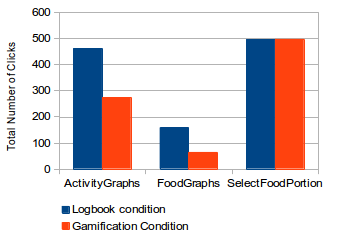
\includegraphics[width=0.6\textwidth]{Figures/self_monitoring_usage.png}
    \rule{35em}{0.5pt}
  \caption{Total clicks on feedback features for self-monitoring of wellness: ``Logbook App'' versus ``Gamified App''.}
  \label{figure:self_monitoring_usage}
\end{figure}\newline
\begin{figure}[htbp]
  \centering
    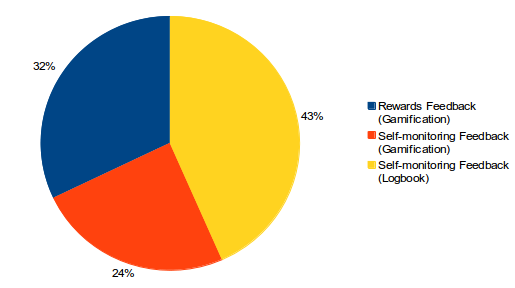
\includegraphics[width=0.45\textwidth]{Figures/clicks_distr.png}
    \rule{35em}{0.5pt}
  \caption{Total clicks on feedback features in the two experimental conditions : self-monitoring features versus rewards features.}
  \label{figure:clicks_distr}
\end{figure}\newline
From Figure \ref{figure:clicks_distr}, we can see that gamification condition's clicks on feedback features are distributed between the main self-monitoring and virtual rewards features. The number of clicks on the main self-monitoring feedback features had decreased as users became interested to feedbacks provided by virtual rewards features more than the main self-monitoring features. This explanation also supplements the reason why usage on Figure \ref{figure:usagedailysessions} above shows the drop on Logbook condition as users who had been exposed gamification condition before logbook condition became less interested with the "Logbook App" after being switched to it. I expanded on this usage phenomenon by examining through baseline data. However, the baseline data such as demographic information were not statistically sufficient to explain the above usage but we can use that information to explain the aforementioned usage trend. The drop in the total number of logbook sessions appears slightly the same in both younger and older intermediaries as shown on Figure \ref{figure:logbookbyage}.  But contrary to this is that younger intermediaries had slightly higher average on total number of sessions compared to the older ones while in gamification condition  as shown on Figure \ref{figure:gambyage}. Also on the average of total number sessions in both experimental conditions, the trend on average shows that younger intermediaries to have more sessions in overall as shown on Figure as more sessions were from gamification condition.  The term old and young are defined by the age \textgreater= and \textless median age (15.5 years old) respectively.  Although the total number of sessions is relative to the number of days in which a pair of users had a particular experimental condition available to them, but young and old intermediaries were evenly distributed to both experimental sequences (LG and GL groups). This means young and old intermediaries were both present in almost the same number in both experimental sequences hence their differences in number sessions which  is influenced by the number of days are expected to cancel each other. The distribution by age group is presented on Table \ref{table:agregroupsall}.\newline 
\begin{figure}[htbp]
  \centering
    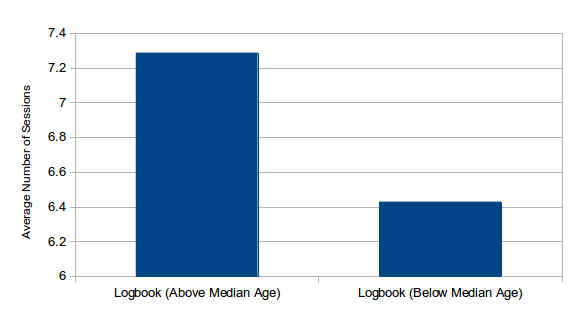
\includegraphics[width=0.5\textwidth]{Figures/logbookbyage.png}
    \rule{35em}{0.5pt}
  \caption{Average number of logbook sessions on  14 intermediaries: Age \textgreater= median age(=15.5) versus Age \textless median age.}
  \label{figure:logbookbyage}
\end{figure}\newline
\begin{figure}[htbp]
  \centering
    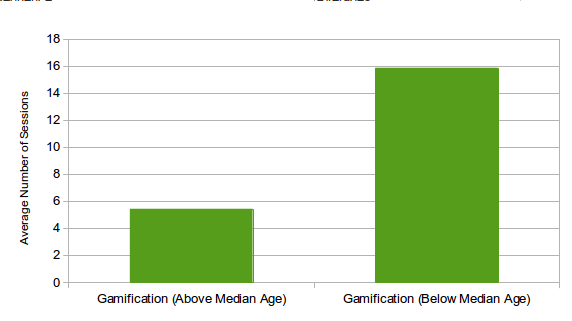
\includegraphics[width=0.5\textwidth]{Figures/gambyage.png}
    \rule{35em}{0.5pt}
  \caption{Average number of gamification sessions on  14 intermediaries: Age \textgreater= median age(=15.5) versus Age \textless median age.}
  \label{figure:gambyage}
\end{figure}\newline
\begin{figure}[htbp]
  \centering
    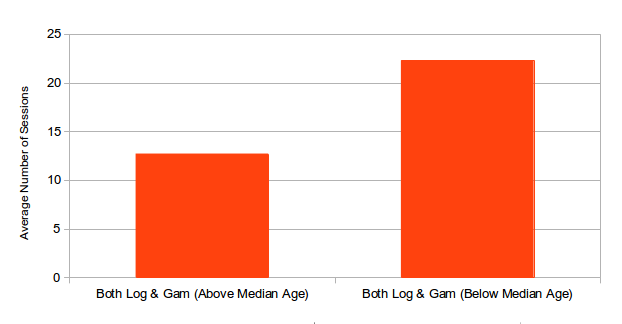
\includegraphics[width=0.5\textwidth]{Figures/bothexpebyage.png}
    \rule{35em}{0.5pt}
  \caption{Average of total number of sessions of  14 intermediaries on both experimental conditions: Age \textgreater= median age(=15.5) versus Age \textless median.}
  \label{figure:bothexpebyage}
\end{figure}
\begin{table}[h!]
  \begin{center}
    \caption{Age groups of intermediary participants}
    \label{table:agregroupsall}
	\begin{tabular}{|c|L{3.2cm}|L{1cm}|L{2cm}|L{2cm}|L{1.6cm}|L{1.3cm}|}
    		\hline
         &\textbf{Age Groups}&\textbf{Total users}&\textbf{No. of GL sequence}&\textbf{No. of LG sequence}&\textbf{No. of Females}&\textbf{No. of Males}\\
         \hline
         1&Age \textgreater=15.5 years&7&3&4&4&3\\  
\hline
         2&Age \textless15.5 years&7&4&3&3&4\\  
\hline
	\end{tabular}
  \end{center}
\end{table}\newline
If we recall about users who had usage problems on Table \ref{table:usageproblems},three out of four intermediary users were above the median age and one below age, therefore one would argue that the trend would change. So lets try to remove some pairs of users from the trends on averages from the aforementioned  Figures \ref{figure:logbookbyage} and \ref{figure:gambyage}. As we have seen on pairs A and B, their usage stopped early during the beginning of the experiments. As for Pair C and D, their motivation to use the app was only hindered during the  gamification condition but they had used the app throughout logbook condition in which Pair C's pedometer was not working but since one of them had their pedometer working and the two intermediaries from the these pairs were close, usage problems didn't affect their utilization of the app while they were in logbook condition. Therefore, in the logbook condition, Lets remove pairs A and B only and the new trend on average number of sessions is shown on Figure \ref{figure:logbookbyage_mod}. For the gamification condition, we remove Pairs A,B,C, and D and the new trend on average session is shown Figure \ref{figure:gambyage_mod}. The same trends continue to hold as younger intermediaries appear to have higher average number sessions in gamification condition and lower average number of sessions in logbook condition. We cannot confidently conclude any thing based on these trends but they can recommended to be considered in future work in the conclusion chapter. Koivisto and Hamari \cite{koivisto2014demographic} found that the usage of  a gamified system is highly affected by the novelty effect which is inversely proportional to the age of participants, meaning that highly usage due to the novelty effect may be reported in much younger participants.   
\newline
\begin{figure}[htbp]
  \centering
    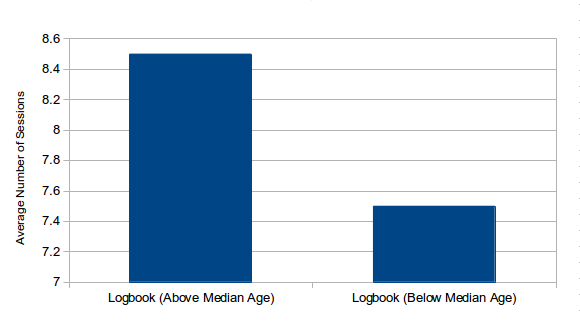
\includegraphics[width=0.5\textwidth]{Figures/logbookbyage_mod.png}
    \rule{35em}{0.5pt}
  \caption{Average number of logbook sessions on  12 intermediaries: Age \textgreater= median age(=15.5) versus Age \textless median age.}
  \label{figure:logbookbyage_mod}
\end{figure}\newline
\begin{figure}[htbp]
  \centering
    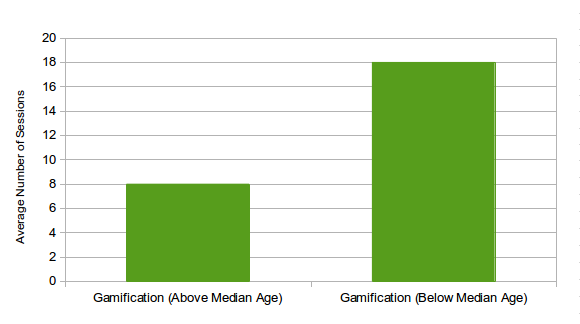
\includegraphics[width=0.5\textwidth]{Figures/gambyage_mod.png}
    \rule{35em}{0.5pt}
  \caption{Average number of gamification sessions on  10 intermediaries: Age \textgreater= median age(=15.5) versus Age \textless median age.}
  \label{figure:gambyage_mod}
\end{figure}\newline
On the next sub sections, user experiences of both intermediaries and beneficiaries are reported .
\subsection{User Experience of Intermediaries}
User experience was analysed through IMI(Intrinsic Motivation Inventory) questionnaires and interviews. The first step was to examine how baseline intrinsic motivation and  demographic information such as age and gender influence user experience. From Figure \ref{figure:bothexpebyage} above, we saw that young intermediaries (age\textless median=15.5 years) appeared to have more number of sessions per day on average, but contrary to this trend is that, at baseline the average perceived enjoyment on helping with cellphone related tasks was higher in intermediaries with age\textgreater=median compared to intermediaries with age\textless median for the 12 intermediary users as shown on Figure \ref{figure:PE_HELP_Age}. 
\begin{figure}[htbp]
  \centering
    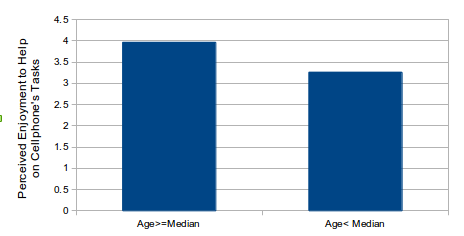
\includegraphics[width=0.5\textwidth]{Figures/PE_HELP_Age.png}
    \rule{35em}{0.5pt}
  \caption{Intermediaries' average perceived enjoyment to help others with cellphone tasks versus age group.}
  \label{figure:PE_HELP_Age}
\end{figure}\newline
I started by comparing the perceived enjoyment to use the family wellness app by age at midline and endline for the 12 intermediary users (excluding users from pairs A and B since they terminated their usage too soon). The purpose of this comparison was to understand why young intermediaries who appeared to be less enjoying on helping with cellphone related tasks, emerged as having more usage sessions than older intermediaries. In this comparison, six intermediary users were below the median age of 15.5 while the remaining six intermediary users were above the median age. More information on these two age groups is provided on Table \ref{table:agegroups}. We can see that both age groups had representatives from both experimental sequences (GL, and LG)  and genders. Figure \ref{figure:PE_Interm_App} shows the averages of perceived enjoyment to use the family wellness app at midline and endline. The averages are higher on the intermediaries with age \textless median for both midline and endline points. \newline
\begin{table}[h!]
  \begin{center}
    \caption{Age groups of intermediary participants}
    \label{table:agegroups}
	\begin{tabular}{|c|L{3.2cm}|L{1cm}|L{2cm}|L{2cm}|L{1.6cm}|L{1.3cm}|}
    		\hline
         &\textbf{Age Groups}&\textbf{Total users}&\textbf{No. of GL sequence}&\textbf{No. of LG sequence}&\textbf{No. of Females}&\textbf{No. of Males}\\
         \hline
         1&Age \textgreater=15.5 years&6&3&3&2&4\\  
\hline
         2&Age \textless15.5 years&6&2&4&4&2\\  
\hline
	\end{tabular}
  \end{center}
\end{table}\newline 
\begin{figure}[htbp]
  \centering
    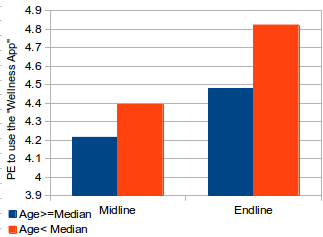
\includegraphics[width=0.5\textwidth]{Figures/PE_Interm_App.png}
    \rule{35em}{0.5pt}
  \caption{Intermediaries' average perceived enjoyment in using the app versus age group.}
  \label{figure:PE_Interm_App}
\end{figure}\newline
There several factors that influence intermediaries to use the app and these are:
\begin{enumerate}
\item{\textbf{Self-monitoring task}}: The task itself of self-monitoring without rewards sparked interests of some intermediary users. This might be as the result of the novelty effect of visualization mechanisms. For instance one intermediary user who happened to be the youngest among all intermediaries reported the highest perceived enjoyment during logbook condition compared to other intermediary users. In addition it seems the phone also had an impact on triggering her interests.
\item{\textbf{Informal comparisons}}: Comparison on steps graphs can be another source motivation. For intermediaries who were close, they did this form of informal comparison. In the absence of gamification, still intermediaries thought that they were competing with other therefore those who were close had face to face interactions of where they did comparison with one another. 
\item{\textbf{Gamification comparison}}: This kind of comparison increased the number of times intermediary user checked the app.
 The ``Gamified App'' was designed in such a way that a pair will earn rewards based on usage and the average number of steps walked by a beneficiary participant who is a member of the pair. The purpose of rewards was to foster users' intrinsic experiences such as competitiveness and a sense of autonomy which are predictors of intrinsic motivation. Rewards depended on four parameters and these were the number of steps walked by a beneficiary user, the number of days the app has been used by an intermediary to either to record meals or to view feedback on meals, points, steps, gardens, etc. During interviews, I discovered that in one pair not only the beneficiary was using the pedometer, an intermediary was also taking turns to use the pedometer, therefore they were collaborating in accumulating steps. Both an intermediary user and a beneficiary user had discussions of whether the person whose turn it was had walk enough steps. They did this to accumulate more steps than other pairs.
\item{\textbf{Requests from beneficiary users}}:There were times where intermediary users engaged with the app only upon receiving requests from beneficiaries. 
\end{enumerate} 
Intermediaries were interested to fulfil requests from beneficiaries provided an intermediary was interested with the self-monitoring task; steps comparison; or gamification comparison. The trend on average perceived enjoyment in both logbook and gamified conditions appeared to be slightly higher in younger intermediaries compared to older intermediaries as shown on Figure \ref{figure:PE_Interm_App_exp_seq}.
\begin{figure}[htbp]
  \centering
    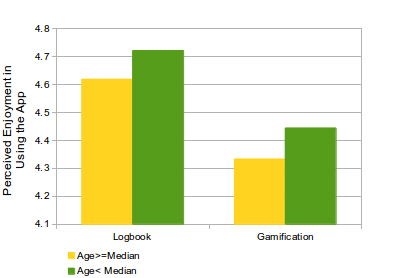
\includegraphics[width=0.5\textwidth]{Figures/PE_Interm_App_exp_seq.png}
    \rule{35em}{0.5pt}
  \caption{Intermediaries' average perceived enjoyment in using the app versus age group (Logbook and Gamification).}
  \label{figure:PE_Interm_App_exp_seq}
\end{figure}\newline
Figures \ref{figure:PE_Interm_App} and \ref{figure:PE_Interm_App_exp_seq}  suggest that the task of helping was more interesting to younger intermediaries due to the existence of the aforementioned motivational affordances.  However, not all intermediaries had positive user experience on utilizing gamification, that is why the average perceived enjoyment appears to be lower for both age groups while in gamification condition compared to the logbook condition. If we go back we can see that four pairs had usage problems as mentioned on Table \ref{table:usageproblems}.  From those four pairs, two pairs had severe usability problems and these were pair A and Pair C. Pair B tried to use the app a few times but since they didn't have data bundles usage was terminated immediately, however, the continued to receive SMS feedback throughout the experimental conditions of which some of it was positive as they had managed to attain some badges. User from pair D also appeared to be more interested during gamification even though he terminated usage after his first week on gamification.  We can see that problems in this pair only started on the fourth week of logbook condition (one week before switching to gamification condition), therefore, the  with the pedometer didn't affect much the motivation of the intermediary user from Pair D as he enjoyed the gamification condition despite the fact that he logged in once throughout this experimental condition and the pedometer was not transmitting data to the server. The two users from Pair B and Pair D, had their motivation not affected by usability problems as for Pairs A and C. SMS feedbacks and reminders were sent to all fourteen pairs and this some how engaged users from Pair B and Pair D. During gamification, if a particular pair managed to acquire a new badge, all other pairs were notified through SMS including the pair that had attained a badge. In addition intermediaries were reminded of what has been done and what remains to be done in order to attain higher badges. During logbook condition, intermediaries were notified with SMS of how many steps have been walked by their intermediary so far and they were also reminded that to assist their beneficiaries in monitoring their wellness. Therefore since, usability problems in Pair B and D were not severe as for pairs A and C, and combination of text messages feedbacks, motivation of users in pairs D, and C appeared to be slightly higher in gamification condition compared to logbook condition. From here we can conclude that Pairs A and C motivations during gamification condition were negatively affected by the severe usability problems.\newline 
Gamification condition didn't harm motivation of only users with severe usability problems. There was  a very intriguing phenomenon from two other intermediary users from \textbf{Pair E} and \textbf{Pair F} as mentioned on Table \ref{table:negexprnce}. The two intermediary users had used the app more often in gamification condition  compared to when they were in logbook condition but had reported both lower scores in perceived enjoyment, and perceived competence when in gamified condition compared to when they were in logbook condition. Two of these intermediary users were  in LG and GL groups respectively. I examined the performance of these two users in gamification rewards and discovered that two users never managed to make any progress in attaining a single reward despite their efforts in using the ``Gamified App''. This harmed both their perceived enjoyment and perceived competence to use the "Family Wellness App" while in gamification condition. One of these two intermediary participants sent an SMS to the researcher asking what he was supposed to do in order to advance in badges and he was informed that all the information was specified in their given user manual. In addition, SMS reminders were sent out to all intermediaries to inform them of how far they have gone in achieving rewards and what is remaining in terms of usage and steps in order for them to reach the next badge. Their beneficiary participants were not walking enough steps despite the fact that these intermediaries had put  more efforts in using the App during gamification condition. Badges were earned in combination of both the app usage and average number of steps walked by a beneficiary user. One beneficiary who was working with one of these intermediary users also reported in interviews that there was always a contention with her intermediary when this beneficiary wanted to see what was going in the app as the intermediary was not voluntarily willing to help some of the time.\newline
\begin{table}
  \begin{center}
    \caption{Pairs affected by poor design of gamification}
    \label{table:negexprnce}
	\begin{tabular}{|l|l|l|l|l|L{6cm}|}
		\hline
		&Pair& Experimental Sequence&No. of logbook sessions/day&No. of gamification sessions/day&Challenge\\
		\hline
		1&Pair E&LG group & The beneficiary participant was not walking enough steps hence impacted performance in gamification\\
		\hline
		2&Pair D & LG group.& Same as above.\\
	\hline
	\end{tabular}
  \end{center}
\end{table}
\newline   
Therefore the conclusion was that, the two intermediary users on Table \ref{table:negexprnce}  had a negative experience as the result of failure of our gamification design to match challenges with abilities. i.e. efforts of beneficiaries differed hence challenges should have matched with individual abilities of beneficiaries within pairs. When challenges are too difficult as they don't match users' skills, end users can become demotivated \citep{zhang2008motivational}. As result only eight intermediary users were considered in the main sub scales of intrinsic motivation (autonomy, competence, and enjoyment).\newline
I compared between the logbook and gamification scores from an IMI questionnaire that assessed intrinsic motivation of intermediaries at midline and endline in using the ``The Family Wellness App''. This questionnaire had four sub-scales which where perceived competence, perceived autonomy,perceived enjoyment, and perceived relatedness.  For the reason stated above, I decided to exclude users from  Pair A and C on Table \ref{table:usageproblems} , and Pairs E and F on Table \ref{table:negexprnce}. A total of ten pairs were considered for analysis of on the aforementioned intrinsic motivation sub-scales.\newline
The hypotheses of interest for intermediaries were:
\begin{enumerate}
\item{Hypothesis 1}
\begin{itemize}
\item{H\SB{0}}:There is no difference in perceived competence in using the app between a logbook app and gamified app
\item{H\SB{A}}:There is a difference in perceived competence in using the app between a logbook app and gamified app
\end{itemize}
\item{Hypothesis 1}
\begin{itemize}
\item{H\SB{0}}:There is no difference in perceived autonomy in using the app between a logbook app and gamified app
\item{H\SB{A}}:There is a difference in perceived autonomy in using the app between a logbook app and gamified app
\end{itemize}
\item{Hypothesis 3}
\begin{itemize}
\item{H\SB{0}}:There is no difference in perceived enjoyment in using the app between a logbook app and gamified app
\item{H\SB{A}}:There is a difference in perceived enjoyment in using the app between a logbook app and gamified app
\end{itemize}
\item{Hypothesis 4}
\begin{itemize}
\item{H\SB{0}}:There is no difference in perceived relatedness in using the app between a logbook app and gamified app
\item{H\SB{A}}:There is a difference in perceived relatedness in using the app between a logbook app and gamified app
\end{itemize}
\end{enumerate}
The results on perceived competence, perceived autonomy,perceived enjoyment, and perceived relatedness of between the ``Logbook App''  and the ``Gamified App'' are shown on Table \ref{table:imiwellnessinterm}. The distribution of the differences of all the scores from the four aforementioned sub-scales, followed a normal distribution hence met a condition for using a paired student t-test.\newline
\begin{table}[h!]
  \begin{center}
    \caption{Comparison of ten intermediaries' scores on sub-scales of competence, autonomy, enjoyment, and relatedness in using the ``Family Wellness App}
    \label{table:imiwellnessinterm}
	\begin{tabular}{|c|c|c|}
		\hline
		Mean &Logbook App&Gamified App\\
		\hline
		 \multirow{2}{*}{Perceived competence}&M=5.23; SD=1.02&M=5.96; SD=0.66\\\cline{2-3} 

		 &\multicolumn{2}{|l|}{t(9)=-3.4949; p=0.0068 ; 95\% CI= -1.204 to -0.258} \\
\hline
		 \multirow{2}{*}{Perceived autonomy}&M=3.95; SD=0.86&M=3.96; SD=0.94\\\cline{2-3} 

		 &\multicolumn{2}{|l|}{t(9)= -0.0269; p= 0.9792; 95\% CI= -0.596 to 0.582} \\
\hline
		 \multirow{2}{*}{Perceived enjoyment}&M=4.18; SD=1.11&M=4.75; SD=1.32\\\cline{2-3} 

		 &\multicolumn{2}{|l|}{t(9)=-1.6930;  p=0.1247; ; 95\% CI= -1.343 to 0.193 } \\
\hline
		 \multirow{2}{*}{Perceived relatedness}&M=4.22; SD=0.63&M=4.37; SD=0.9\\\cline{2-3} 
		 &\multicolumn{2}{|l|}{t(9)= -0.7193; p=0.4902; 95\% CI= -0.622 to 0.322 } \\
\hline
	\end{tabular}
  \end{center}
\end{table}
\newline
Perceived competence of intermediaries in using the ``Family Wellness App'' was significantly higher in the gamified condition than in the logbook condition in the ten intermediaries that were analysed. Perceived autonomy, perceived enjoyment, and perceived relatedness were all not different between gamification condition and logbook condition. For perceived enjoyment and autonomy, there are cases were the self-monitoring task was interesting enough on itself or when combined with informal comparison of steps among intermediary users. Therefore, there some intermediaries who felt more enjoyment while they were in logbook condition, which is also the same case for perceived autonomy. For perceived relatedness, the app brought users together regardless of an experimental condition especially the ones that already knew each other before.  \newline
\subsection{Beneficiaries' IMI Scores on Health Self-Monitoring}
I used the IMI (intrinsic motivation inventory) questionnaire to assess motivation of intermediaries in self-monitoring of Diet. I excluded pairs (A,B, C, and D) from Table \ref{table:usageproblems} problems that led discontinuation of usage. In total only ten out of fourteen beneficiaries had their results included for analysis. We have seen from the sub section (\ref{methodsquestionnaire}) that this questionnaire was administered at baseline, midline and endline.\newline
In the first comparison,I compared the IMI score of each participant at baseline, midline, and endline regardless of the experimental condition. In the second comparison I compared scores at baseline, logbook, and gamification condition. The IMI score was computed from the average of all scores from sub-scales of perceived competence, perceived autonomy, perceived relatedness, perceived enjoyment, perceived effort,  and perceived usefulness. I  used one way ANOVA with repeated measures to test if there a difference  between scores at: (1) baseline, midline, and endline, and (2)baseline, logbook and gamification. I used Mauchy's test\footnote{Read more on how Mauchy's test is used from http:/Business analysis attempts to study the exsting market. /www.statisticshell.com/docs/repeatedmeasures.pdf} to check if baseline,midline and endline scores had the same covariance in each ANOVA test I carried out and this helped in deciding of what correction to use on SPSS results among ``Sphericity Assumed'',``Greenhouse-Geisser'', and ``Huynh-Feldt'' as reported on the next sub-sections.
\subsubsection{IMI in Self-Monitoring of Diet}
The results on self-monitoring of diet (baseline, midline, and endline) are shown on Table  \ref{table:imidietbenf}. The Mauchly’s test indicated that the assumption of sphericity was not violated with  $\chi{}$\SP{2}(2)=3.76, p=0.152.\newline
\begin{table}[h!]
  \begin{center}
    \caption{Comparison of ten beneficiaries' IMI scores in self-monitoring of diet at baseline, midline and endline}
    \label{table:imidietbenf}
	\begin{tabular}{|L{2.8cm}|L{3.2cm}|L{3.2cm}|L{3.2cm}|}
		\hline
		Mean IMI Score &Baseline&Midline&Endline\\
		\hline
		 %\multirow{3}{*}
		 {Self-monitoring}&M=4.48; SD=1.24&M=5.07; SD=1.19;&M=5.55; SD=0.95\\\cline{2-4} 

		of Diet &\multicolumn{3}{|l|}{F(2,18)=3.787; p=0.042} \\
\hline	\end{tabular}
  \end{center}
\end{table}\newline
Therefore, the results (N=10) on  ``Self-monitoring of Diet'' shown on Table \ref{table:imidietbenf} were from ``Sphericity Assumed'' output. ANOVA showed that there was a significant difference of average IMI scores on self-monitoring of diet measured at baseline, midline and endline.\newline
I further conducted a student t-test to see if there was difference in IMI scores to self-monitor diet by contrasting the following: (1) baseline versus midline; (2) baseline versus endline; and (3) midline versus endline. The results are shown on Tables \ref{table:imipairwisediet}, \ref{table:imipairwisediet1}, and \ref{table:imipairwisediet2}. There was a significant difference between IMI scores on baseline versus endline but not on baseline versus midline and midline versus endline. Motivation to self-monitor diet appeared to increase with time as shown on Figure \ref{figure:imi_diet}. The interpretation of the above findings are that the wellness app appears to have a significant effect with time on motivation of beneficiaries to self-monitor their diet.
\begin{table}[h!]
  \begin{center}
    \caption{Pairwise comparisons of IMI scores in self-monitoring of diet: Baseline versus Midline}
    \label{table:imipairwisediet}
	\begin{tabular}{|L{2cm}|L{4cm}|L{4cm}|}
		\hline
		Mean &Baseline&Midline\\
		\hline
		 \multirow{2}{*}{IMI Score}&M=4.48; SD=1.24&M=5.07; SD=1.19\\\cline{2-3} 

		 &\multicolumn{2}{|l|}{t(9)=-1.298; p=0.227 ; 95\% CI= -1.621 to 0.439} \\
\hline
	\end{tabular}
  \end{center}
\end{table}
\begin{table}[h!]
  \begin{center}
    \caption{Pairwise comparisons of IMI scores in self-monitoring of diet: Baseline versus Endline}
    \label{table:imipairwisediet1}
	\begin{tabular}{|L{2cm}|L{4cm}|L{4cm}|}
		\hline
		Mean &Baseline&Endline\\
		\hline
		 \multirow{2}{*}{IMI Score}&M=4.48; SD=1.24&M=5.55; SD=0.95\\\cline{2-3} 

		 &\multicolumn{2}{|l|}{t(9)=-2.457; p=0.036 ; 95\% CI= -2.06083 to -0.08517} \\
\hline
	\end{tabular}
  \end{center}
\end{table}
\begin{table}[h!]
  \begin{center}
    \caption{Pairwise comparisons of IMI scores in self-monitoring of diet: Midline versus Endline}
    \label{table:imipairwisediet2}
	\begin{tabular}{|L{2cm}|L{4cm}|L{4cm}|}
		\hline
		Mean &Midline&Endline\\
		\hline
		 \multirow{2}{*}{IMI Score}&M=5.07; SD=1.19&M=5.55; SD=0.95\\\cline{2-3} 

		 &\multicolumn{2}{|l|}{t(9)=-1.975; p=0.08 ; 95\% CI= -1.0342 to 0.07017} \\
\hline
	\end{tabular}
  \end{center}
\end{table}
\newline
\begin{figure}[htbp]
  \centering
    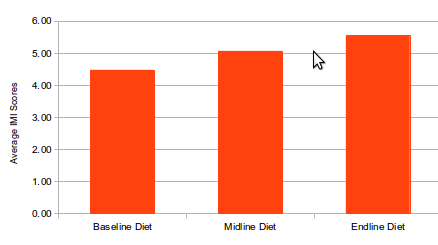
\includegraphics[width=0.4\textwidth]{Figures/imi_diet.png}
    \rule{35em}{0.5pt}
  \caption{Trend on Average IMI Scores of Self-Monitoring of Diet at Baseline, Midline, and Endline.}
  \label{figure:imi_diet}
\end{figure}\newline
The aforementioned ANOVA comparison among baseline, midline, and endline doesn't discern between different experimental conditions of which pairs of users were exposed to. The second task was to examine the comparison on IMI scores to self-monitor diet, among baseline, logbook, and gamification conditions. The ANOVA results (N=10) are shown on Table  \ref{table:imidietbenf2}. I chose the ``Sphericity Assumed'' output of the ANOVA test since the Mauchly’s test indicated that the assumption of sphericity was not violated with  $\chi{}$\SP{2}(2)=2.19, p=0.335. Therefore, the results on  ``Self-monitoring of Diet'' shown on Table \ref{table:imidietbenf2} were from ``Sphericity Assumed'' output. ANOVA showed that there was no significant difference of average IMI scores on self-monitoring of diet measured during baseline, logbook and gamification conditions. The trend on averages shows both logbook and gamification to be slightly higher than baseline as shown on Figure \ref{figure:imi_diet2}. The conclusion from this finding is that is that both versions of the prototype have show an indication of increasing motivation of beneficiaries to self-monitor diet. However, the logbook condition achieved a significant result. In the informative evaluation that was conducted before this evaluation, it was found out that beneficiary users tended to give more value to the main feedback features for self-monitoring of steps and diet \citep{katule2016leveraging}, while in the Figure \ref{figure:self_monitoring_usage} above we saw that the trend on utilization of the main feedback features for self-monitoring of steps and diet decreased during gamification condition. This could be one of the reasons of why we achieved a significant result only on logbook when compared to baseline and not on gamification when compared to baseline. Another explanation is attributed to the our smaller sample sizes hence the power of the effect size is reduced.\newline
\begin{table}[h!]
  \begin{center}
    \caption{Comparison of ten beneficiaries' IMI scores in self-monitoring of diet at baseline, after logbook, and  after gamification conditions}
    \label{table:imidietbenf2}
	\begin{tabular}{|L{2.8cm}|L{2.5cm}|L{2.5cm}|L{2.5cm}|}
		\hline
		Mean IMI Score &Baseline&Logbook&Gamification\\
		\hline
		 %\multirow{3}{*}
		 Self-monitoring&M=4.48; SD=1.241&M=5.28; SD=1.05&M=5.34; SD=1.16\\\cline{2-4} 
		 of Diet&\multicolumn{3}{|l|}{F(2,18)=3.787; p=0.087} \\
\hline	\end{tabular}
  \end{center}
\end{table}\newline
\begin{figure}[htbp]
  \centering
    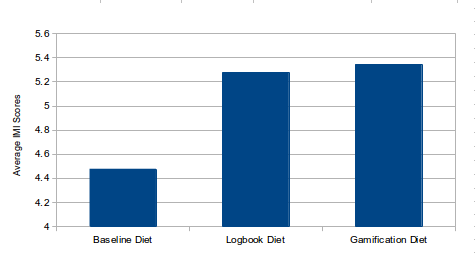
\includegraphics[width=0.4\textwidth]{Figures/imi_diet2.png}
    \rule{35em}{0.5pt}
  \caption{Trend on Average IMI Scores of Self-Monitoring of Diet at Baseline, Logbook, and Gamification.}
  \label{figure:imi_diet2}
\end{figure}\newline
\subsubsection{IMI in Self-Monitoring of Activity}
The results (N=9) on self-monitoring of activity are shown on Table  \ref{table:imiactivitybenf}. The results are based on a sample of nine beneficiary users as one participant didn't complete this part of the questionnaire at baseline.  The Mauchly’s test indicated that the assumption of sphericity was violated with  $\chi{}$\SP{2}(2)=8.248, p=0.016. The value $\epsilon$ on Greenhouse Geisser was ``\textless 0.75'', therefore, the results on  ``Self-monitoring of Diet'' shown on Table \ref{table:imiactivitybenf} were selected from ``Greenhouse-Geisser'' output. ANOVA showed that there was no significant difference of average IMI scores on self-monitoring of activity measured at baseline, midline and endline. The trend of means appears to increase from baseline to endline as shown on Figure \ref{figure:imi_activity}. There are several factors that could have contributed to results not being significant among baseline, midline,endline points,. The first hypothesized reason is tracking of of physical activity appeared to be easy in majority of the participants even without tracking devices as people can estimate the distance they walk daily and they consider this as tracking even though they might have means to record this information, hence their motivation was high at baseline unlike diet self-monitoring which they consider it to be cumbersome due to external barriers such as health food being expensive, therefore at baseline participants felt more motivated to track their activity. The second hypothesized reason is that the sample size was small hence there was a smaller power in detecting significant difference. But we have seen that the trend in motivation increases with time.\newline 
\begin{table}[h!]
  \begin{center}
    \caption{Comparison of ten beneficiaries' IMI scores in self-monitoring of activity at baseline, midline and endline}
    \label{table:imiactivitybenf}
	\begin{tabular}{|L{2.8cm}|L{2.5cm}|L{2.5cm}|L{2.5cm}|}
		\hline
		Mean IMI Score &Baseline&Midline&Endline\\
		\hline
		 %\multirow{3}{*}
		 Self-monitoring&M=4.82; SD=1.002&M=5.28; SD=1.003&M=5.41; SD=0.894\\\cline{2-4} 
		 of activity&\multicolumn{3}{|l|}{F(1.182, 9.455)=2.936; p=0.116} \\
\hline	\end{tabular}
  \end{center}
\end{table}\newline
\begin{figure}[htbp]
  \centering
    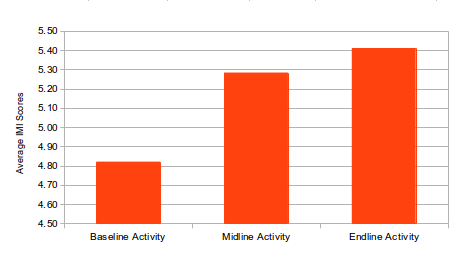
\includegraphics[width=0.4\textwidth]{Figures/imi_activity.png}
    \rule{35em}{0.5pt}
  \caption{Trend on Average IMI Scores of Self-Monitoring of Activity at Baseline, Logbook, and Gamification.}
  \label{figure:imi_activity}
\end{figure}\newline
I conducted another analysis (N=9) to examine if there is a difference among baseline,logbook, and gamification in self-monitoring of activity. The Mauchly’s test indicated that the assumption of sphericity was violated with  $\chi{}$\SP{2}(2)=6.788, p =0.034. The value of $\epsilon$ on Greenhouse Geisser was ``\textless 0.75'', therefore, the results on  ``Self-monitoring of Activity'' shown on Table \ref{table:imiactivity2benf} were selected from ``Greenhouse-Geisser'' output. ANOVA showed that there was no significant difference of average IMI scores on self-monitoring of activity measured at baseline, logbook and gamification.  The same reasons on Table \ref{table:imiactivitybenf}  for not achieving statistical significance are also valid in this case. Also the trend in motivation increases in both logbook and gamification as shown on Figure \ref{figure:imi_activity2}\newline
%epsilon=0.617
\begin{table}[h!]
  \begin{center}
    \caption{Comparison of ten beneficiaries' IMI scores in self-monitoring of activity at baseline, logbook and gamification}
    \label{table:imiactivity2benf}
	\begin{tabular}{|L{2.8cm}|L{2.5cm}|L{2.5cm}|L{2.5cm}|}
		\hline
		Mean IMI Score &Baseline&Logbook&Gamification\\
		\hline
		 %\multirow{3}{*}
		 Self-monitoring&M=4.82; SD=1.002&M=5.33; SD=0.9762&M=5.37; SD=0.9276\\\cline{2-4} 
		 of activity&\multicolumn{3}{|l|}{F(1.234, 9.872)=2.783; p=0.123} \\
\hline	\end{tabular}
  \end{center}
\end{table}\newline
\begin{figure}[htbp]
  \centering
    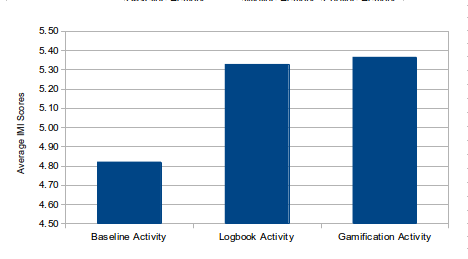
\includegraphics[width=0.4\textwidth]{Figures/imi_activity2.png}
    \rule{35em}{0.5pt}
  \caption{Trend on Average IMI Scores of Self-Monitoring of Activity at Baseline, Logbook, and Gamification.}
  \label{figure:imi_activity2}
\end{figure}\newline
\begin{flushright}
\end{flushright}


%\input{Chapters/Chapter4} 
%\input{Chapters/Chapter5} 
%\input{Chapters/Chapter6} 
%\input{Chapters/Chapter7} 

%----------------------------------------------------------------------------------------
%	THESIS CONTENT - APPENDICES
%----------------------------------------------------------------------------------------

\addtocontents{toc}{\vspace{2em}} % Add a gap in the Contents, for aesthetics

\appendix % Cue to tell LaTeX that the following 'chapters' are Appendices

% Include the appendices of the thesis as separate files from the Appendices folder
% Uncomment the lines as you write the Appendices

%% Appendix A

\chapter{Appendix Title Here} % Main appendix title

\label{AppendixA} % For referencing this appendix elsewhere, use \ref{AppendixA}

\lhead{Appendix A. \emph{Appendix Title Here}} % This is for the header on each page - perhaps a shortened title

Write your Appendix content here.
%\input{Appendices/AppendixB}
%\input{Appendices/AppendixC}

\addtocontents{toc}{\vspace{2em}} % Add a gap in the Contents, for aesthetics

\backmatter

%----------------------------------------------------------------------------------------
%	BIBLIOGRAPHY
%----------------------------------------------------------------------------------------

\label{Bibliography}

\lhead{\emph{Bibliography}} % Change the page header to say "Bibliography"

\bibliographystyle{unsrtnat} % Use the "unsrtnat" BibTeX style for formatting the Bibliography

\bibliography{Bibliography} % The references (bibliography) information are stored in the file named "Bibliography.bib"

\end{document}  